\documentclass[11pt, a4paper,openany]{article}%openany-> remove blank page after part in book

\usepackage[utf8]{inputenc}
%\usepackage{graphicx,verbatim,eurosym,epstopdf,mathtools}
\usepackage{gensymb}
\usepackage[top=3.5cm, bottom=2.5cm, left=2.7cm, right=2.7cm]{geometry}
\usepackage{fancyhdr} 
	\lhead{}
	\chead{}
	\rhead{}
\pagestyle{fancy}
\usepackage[spanish, english]{babel}

\usepackage{tikz}
\usetikzlibrary{calc}
\usetikzlibrary{positioning}
\usetikzlibrary{matrix}

\usepackage{tikz}
\usetikzlibrary{arrows}

\usepackage{titlesec}

 
\usepackage{float} %change floating behaviour of figures8
\usepackage{caption}
\usepackage{subcaption}%figures side-byside
\usepackage{listings} %include code
\usepackage{pdfpages} %include complete pdfs
\pgfdeclarelayer{background}
\pgfsetlayers{background,main}

\usepackage{sectsty}%change code of part,section...
\partfont{\color{part}}
\sectionfont{\color{section}}
\subsectionfont{\color{subsection}}
\subsubsectionfont{\color{subsubsection}}
\definecolor{part}{HTML}{304EA1}
%subsection 3E65CF
%subsubsection 4570E6
\definecolor{section}{HTML}{375AB8}
\definecolor{subsection}{HTML}{3E65CF}
\definecolor{subsubsection}{HTML}{4570E6}


\usepackage[]{hyperref}%hyperlinks [hidelinks]
\hypersetup{
 colorlinks,
 citecolor=blue,
 citebordercolor=white,
 linkbordercolor=white,
 linkcolor=black,
 urlcolor=blue
 }



\usepackage{graphicx}

\def\mathLarge#1{\mbox{\Large $#1$}} %Define the size of fractions

%<code citing>%
\usepackage{color}
\usepackage{xcolor}
\usepackage{listings}
\usepackage{caption}
\DeclareCaptionFont{white}{\color{white}}
\DeclareCaptionFont{gray}{\color{gray}}
\DeclareCaptionFormat{listing}{\colorbox{gray}{\parbox{15cm}{#1#2#3}}}%\textwidth}{#1#2#3}}}
\captionsetup[lstlisting]{format=listing,labelfont=white,textfont=white}
%</code citing>%

\usepackage{enumerate}% list with roman numerals

\usepackage{float}%to put figures in minipage

\usepackage[titletoc, title]{appendix}%appendix to toc

\usepackage[official]{eurosym}%use the euro symbol 



\begin{document}

% PORTADA 
\begin{titlepage}

\begin{center}


% HEADER

\includegraphics[width=0.25\textwidth]{images/uc3m.jpg}\\[2cm]    
\textsc{\huge University Carlos III of Madrid}\\[0.5cm]
\textsc{\Large Industrial Electronics and Automation Engineering}\\[0.5cm]
\textsc{\large Bachelor Thesis}\\[4cm]

% TÍTULO
{\LARGE \bfseries{Design, construction and programming of a low cost, Open Source robot for assistive activities}\\[4.5cm]}
 
 
\end{center}
% AUTORES Y SUPERVISORES

\begin{minipage}{0.55\textwidth}
\begin{flushleft} \large
\emph{Author}\\
Alvaro Ferrán Cifuentes\\

\end{flushleft}
\end{minipage}
\begin{minipage}{0.4\textwidth}
\begin{flushright} \large
\emph{Supervisor}\\
Juan González Víctores

\end{flushright}\end{minipage}\vfill

\vfill











%\vfill

% FOOTER




\end{titlepage}

\setlength{\parindent}{0cm}

\selectlanguage{english}

\newpage
\pagenumbering{gobble}% Remove page numbers (and reset to 1)

\vspace*{2cm}
\color{part} \textsc{\Large \textbf{Acknowledgemts}}\\[0.5cm]
\color{black}
First of all, I would like to thank my parents for their unwavering support.\\

I want to acknowledge Irene, for her support, interest and help throughout the project.\\

I want to acknowledge my tutor, Juan González Víctores, for the time and help put into this project, and for enabling me to carry it out.\\

I want to thank as well both Alberto Valero and Juan González Gómez for their enthusiastic approach to teaching and for the ``Mars Challenge" project, throughout which they initiated me into the world of robotics and 3D printing.\\

Finally, I would like to thank my familly and friends for always being there when needed.\\[1cm]

\vspace*{1cm}
\color{part} \textsc{\Large \textbf{Agradecimientos}}\\[0.5cm]
\color{black}

Antes de nada quiero agradecer a mis padres el apoyo que me dan siempre. \\

En primer lugar, un reconocimiento especial a Irene por su apoyo, interés y ayuda a lo largo del proyecto.\\

Agradezco también a mi tutor, Juan González Víctores, el tiempo y la ayuda prestados para la realización de este trabajo, así como por habilitarlo para que pudiera desarrollarlo.\\

Así mismo, agradezco a Alberto Valero y a Juan Gonzáĺez Gómez su entusiasmo por la docencia y por el proyecto ``Mars Challenge", a través del cual me embarcaron en el mundo de las impresoras 3D y de la robótica.\\

Por último quiero dar las gracias a mi familia y amigos, por estar siempre ahí cuando se les necesita.
























































\color{black}


\newpage
\pagenumbering{gobble}% Remove page numbers (and reset to 1)

\vspace*{2cm}
\begin{center}
\color{part} \textsc{\huge \textbf{Abstract}}\\[1cm]
\end{center}

The average age of developped countries is increasing and will tend to do so even more in the future. With a growing number of elderly people needing assistance, the demand for aid is rapidly outgrowing the supply available.\\

In order to reverse this situation, personal robots capable of assisting people both emotionally and physically are being developed. These robots will be able to take care of the elders' needs and being artificial helpers, enough of them can be fabricated to satisfy the demand.\\

In this project an assistive robot prototype is developped. While being relatively small in size, it is programmed taking into account that the software will eventually be ported to a full-sized robot, and so it has the same capabilities.\\

The Personal Domestic Service Droid (PD-SD) has a humanoid upper-body attached to a wheeled base. It has two arms with five degrees of freedom each which are used to grab objects or perform actions such as closing doors, while the differential-drive base enables it to maneuver in small spaces since it is capable of rotating in place.\\

The PD-SD is controlled from an Android phone over a wireless network it creates. The application enables the user to control each of the arm actuators separately or in couples, moving symmetrical motors together. Additional controls include a directional pad to control the base motors, a button for closing or opening the grippers and a button to go back to the initial position. Finally, the top half of the screen is reserved to displaying video received from the on-board camera.\\

On the robot itself, a Raspberry Pi computer acts as the brains. It enables the wifi network and receives the orders through it, as well as streaming video to the phone. All of the previous is scripted, so it completes the tasks automatically when turned on.\\

When a connection between Android and Raspberry has been achieved the LCD will display a message informing the user of this, and will do the same when the connection is lost. The data received is sent through serial port to an Arduino microcontroller which will then parse the message and control the different actuators. 
\newpage
\pagenumbering{gobble}% Remove page numbers (and reset to 1)
\vspace*{2cm}

\begin{center}
\color{part} \textsc{\huge \textbf{Resumen}}\\[1cm]
\end{center}


La edad media de los países desarrollados está aumentando, y tenderá a hacerlo aún más en el futuro. Con un número cada vez más importante de personas mayores con necesidad de asistencia, la demanda de ayuda está sobrepasando rápidamente la oferta disponible.\\

Para revertir la situación están siendo desarrollados robots capaces de asistir personas tanto emocional como físicamente. Estos robots satisfacerán las necesidades de los mayores, y siendo ayudantes artificiales se podrán construir los suficientes para satisfacer la demanda.\\

En este proyecto se desarrolla un prototipo de robot asistencial. A pesar de su tamaño relativamente pequeño, está programado teniendo en cuenta que el código se portará más adelante a un robot de tamaño humano, y por tanto es capaz de realizar lo mismo.\\

El Droide de Servicio Doméstico Personal (PD-SD por sus siglas en inglés) tiene un torso con brazos humanoide acoplado a una base con ruedas. Tiene dos brazos, cada uno con cinco grados de libertad que pueden ser utilizados para coger objetos o realizar acciones como cerrar puertas, mientras que la base móvil diferencial le permite maniobrar en espacios pequeños, ya que es capaz de rotar en el sitio.\\

El PD-SD se controla desde un teléfono con Android a través de una red wifi. La aplicación permite el control individual o por parejas simétricas de los motores de los brazos. Además permite controlar la base mediante un pad direccional, tiene un botón para abrir o cerrar las pinzas y otro para llevar al robot a su posición inicial. Finalmente, la parte superior de la pantalla está reservada para reproducir el vídeo recibido de la cámara de abordo.\\

En el propio robot un ordenador Raspberry Pi actúa de cerebro. Crea la red wifi a través de la cual recibe las órdenes y retransmite por ella el vídeo. Todo lo anterior está incluido en un script, con lo que se realiza automáticamente al encender el robot.\\

Cuando se establece una conexión entre el teléfono y el ordenador la pantalla LCD informará de ello mediante un mensaje, y hará lo propio cuando la conexión se cierre. Los datos recibidos se reenviarán mediante el puerto serie a un Arduino, que los parseará y controlará los actuadores pertinentes.
\newpage
\pagenumbering{roman} 
\tableofcontents
\clearpage
\listoffigures 
\clearpage
\lstlistoflistings
\clearpage

\pagenumbering{arabic}
% Intro
%\part{Introduction} 
\section{Introduction}

The Merriam-Webster dictionary defines a robot as ``a machine that can do the work of a person and that works automatically or is controlled by a computer". From the purely mechanical Renaissance automata, like the walking and praying monk in the Smithsonian Instute's collection\cite{automata-monk}  to the state of the art ASIMO, referenced in the following chapter, robots have always spurred the collective imagination and enthusiam of their builders.\\
	
	
From the mid-twentieth century the robot universe has vastly expanded, and they are now present in almost every field, ranging from construction\cite{robot-construction} to space\cite{robot-space} or medicine\cite{robot-medicine}. However, a new type of robot is beginning to appear: the domestic robot. This can be either purely social, limited to interacting and connecting emotionally with people\cite{robot-social} or assistive, designed to carry out tasks a person needs help with\cite{jardon2011personal}.\\

Until now, most assistive robots were limited to specific tasks, like helping with feeding or transporting people. This proyect however intends to build a general purpose assistive robot, that users can telecontrol from their phones and later on program simple routines to be repeated at a certain frequency.


\subsection{Socio-economic factors}

Developped countries' populations are ageing. With improved health systems the average life expectancies are getting higher. In Spain this situation is even more noticeable, since in a study by realized by the World Health Organization (WHO) \cite{who-life} it is shown that Spaniard women have the highest life expectancy in Europe and the second highest in the world, only behind Japan.\\

While increasing life expectancies is a victory for individuals, combined with lowering birth rates results in average population age increments. This means that there will be more elder people depending on the younger generations and not enough of the latter to help them in daily activities.
With the actual trend of continuously increasing life expectancies in Europe \cite{life-future}, the situation in those countries will be even more pronounced.\\

One solution may be to include social, domestic robots that would assist with domestic chores. The proposed solution tries to tackle this problem by doing exactly that: a low cost robot that anybody can buy or build and improve as needed.\\

The components are chosen taking into account reach and cost. The controller is an Android smartphone, since up to 66 percent of the population in Spain owns a smartphone\cite{numero-smartphone}, and out of those around 85 percent are Android\cite{numero-android}. Android phones also come in all prices, so users without a phone can buy the least expensive models and still be able to use the robot.\\

The on-board electronic brains, a computer and a microcontroller board are a Raspbery Pi and an Arduino respectively. These have been chosen for their capabilities, but especially for their price tags: the former costs 40\euro  and the second 23\euro, far below the 300\euro price line most ``cheap" computers cost.\\

Finally, the robot parts are 3D printed, since that is much more cost-efficient in small batches than mold injection, especially for an evolving product like a robot improved by the user community.


\subsection{Proposed solution}
The proposed solution is the creation of a Personal Domestic Service Droid (PD-SD), a robot with a humanoid upper body on a wheeled base that will be capable of assisting elderly people or with physical dissabilities. While the final robot should be of full human-size, to be able to lower high objects, a smaller prototype will be presented in this project. This is done to keep the focus on the software, which is identical and can be exported directly to a full-size robot when it is perfected, while creating a scale model to use while improving the programs.\\

The PD-SD is controlled from the user's Android smartphone, which will connect to the robot's wifi network to control it. The latter will also stream video from its camera to the smartphone, while obbeying the instructions given from the Android application. It has two arms with 5 degrees of freedom each to be able to grasp objects or perform simple actions such as closing doors, and a differential-drive base to move throughout space while being able to rotate in place, which may be useful to avoid getting stuck in small spaces such as corridors.\\










\subsection{Scope of the project}

This project's ultimate objective is to build a robotic assistant prototype, which may be controlled by a user from their own smartphone and which will stream a video feed from its camera so the user is able to see through the robot. This prototype is built to develop the technology that can be later used in a full-scale robot capable of assisting elderly people or with disabilities.\\

In order to achieve this result, the project is divided into the following objectives:

	\begin{enumerate}[I.]

		\item Study of different robot configurations to find the optimal choice for domestic assistive activities.\\

		\item Design of the aforementioned robot.\\

		\item Creation of the designed parts with a 3D printer.\\

		\item Assembly of the robot's body and installation of the electronic components.\\

		\item Program the microcontroller to understand the user's commands and control the actuators accordingly.\\

		\item Program the onboard computer to: 
			\begin{enumerate}[i.] 
			\item set up a wifi network to communicate with the user
			\item stream video from the attached camera 
			\item send the user's commands to the microcontroller.
			\item do all of the previous automatically when the system boots.\\
			\end{enumerate}

	
		\item Program the Android application the user will use to control the robot and receive the video feed it streams.

	\end{enumerate}


% \section{Project phases}
% [include Gantt diagram]

% \section{Components and equipment employed}
% 	The following catalogue contains all the components employed during the scope of the project.

% 	\begin{itemize}

% 		\item \textbf{3D printer}

% 	\end{itemize}
\newpage


% State of the art
%\part{State of the art} 
\section{State of the art}

Robots that interact with humans have been developped since the mid-twentieth century. Here is a list of some of the most relevant robots to the field of application of the PD-SD built to date. 


\subsection{SAM/Robonaut}
Built in 1969, the Self-propelled Anthropomorphic Manipulator (SAM), seen in Figure \ref{sam}, was NASA's first radio teleoperated robot. It was composed of two distinct parts: the manipulator and the control center.\\

The manipulator consisted of a torso with two arms and a camera attached to a four wheeled base. The robot sent video feed from the camera over a radio to the operator which would receive the video on a television set.\\

	\begin{figure}[H]
			\centering
			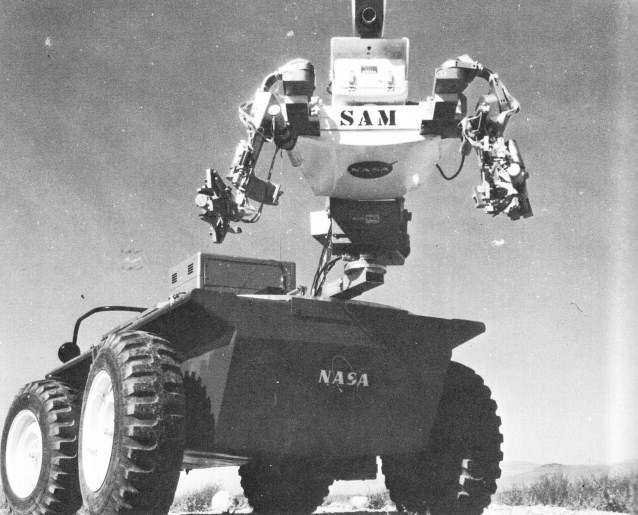
\includegraphics[scale=0.5]{images/StateOfArt/SAM.jpg}
			\caption{NASA's Self-propelled Anthropomorphic Manipulator }
			\label{sam}
	\end{figure}
	\bigskip

The control station, as seen in Figure \ref{sam2}, included an upper-body exoskeleton through which the operator could move their arms and have the robot replicate the movements and the screen through which the robot displayed the video stream.\\

	\begin{figure}[H]
			\centering
			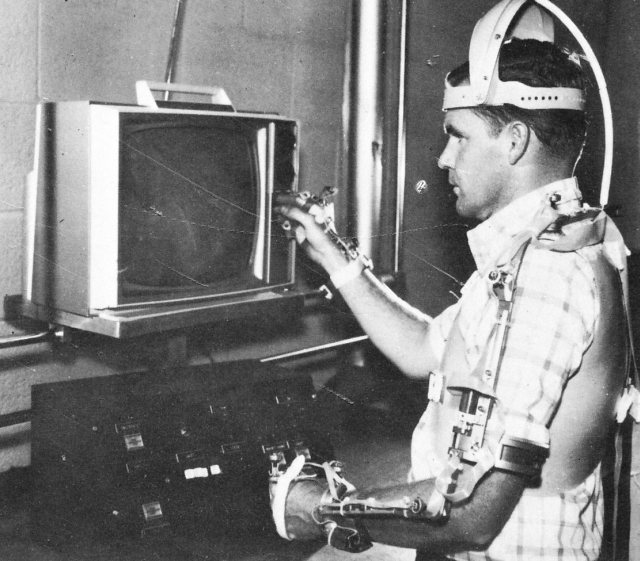
\includegraphics[scale=2]{images/StateOfArt/SAM2.jpg}
			\caption{SAM's control station }
			\label{sam2}
	\end{figure}
	
In the year 1997 NASA started developping Robonaut, a teleopresence robot that would assist astronauts in tasks too dangerous or mundane for them to work on. The combination of the four wheeled base Centaur with Robonaut creates a powerful, efficient, fast successor of the original SAM, while providing a much smaller, portable control station (Figure \ref{robonaut}).

	\begin{figure}[H]
			\centering
			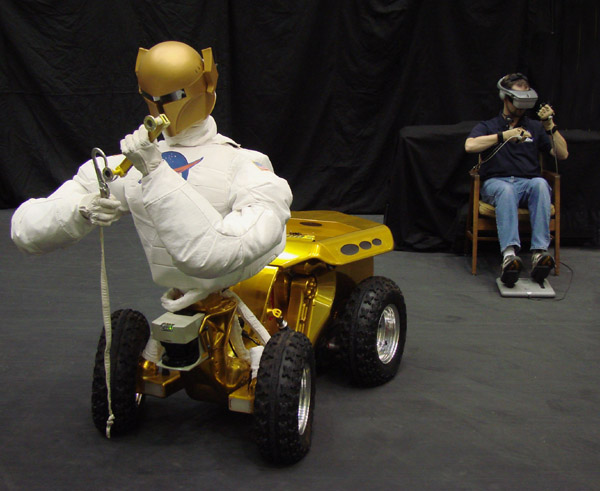
\includegraphics[scale=0.55]{images/StateOfArt/robonaut.jpg}
			\caption{Operator controlling the Robonaut coupled to the Centaur}
			\label{robonaut}
	\end{figure}
	\bigskip 

%\subsection{Asibot}

\subsection{Asimo}

Introduced in the year 2000, Honda's Advanced Step in Innovative MObility (ASIMO) is a humanoid robot designed to assist humans in daily tasks. Its height of 130cm ensures it is able to operate door handles and light switches. Capable of recognizing voice commands and common gestures such as pointing or waving as well as different human faces, the robot is capable of facing and interacting with whoever is speaking. \\


	\begin{figure}[H]
			\centering
			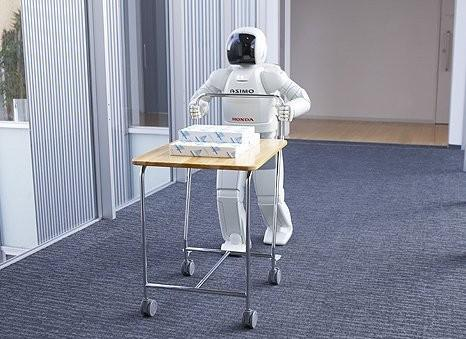
\includegraphics[scale=0.7]{images/StateOfArt/asimo.jpg}
			\caption{ASIMO pushing a cart}
			\label{asimo}
	\end{figure}
	\bigskip

Some of its aditional abilities include navigating space while avoiding oncoming people, carrying or pushing objects (Figure \ref{asimo}), using the stairs, playing sports such as soccer and heading towards its charging station whenever it detects its battery charge level is low.\\

\newpage
\subsection{RIBA}

The Robot for Interactive Body Assistance (RIBA) was developped in conjunction between RIKEN and Tokai Rubber Industries in the year 2004 to provide assistance in human handling, such as setting a person into thei wheelchair or transporting them to their bed.\\

The first RIBA, from 2009, could lift around 60kg, while the new RIBA II from 2011 is able to carry up to 80kg, which would cover most of Japan's population, the average adult weighing around 60kg.\\

Its 140cm height ensures it is able to lift people to the highest beds, while its 180kg provides a solid counterweight to avoid toppling over when carrying a person.\\

	\begin{figure}[H]
			\centering
			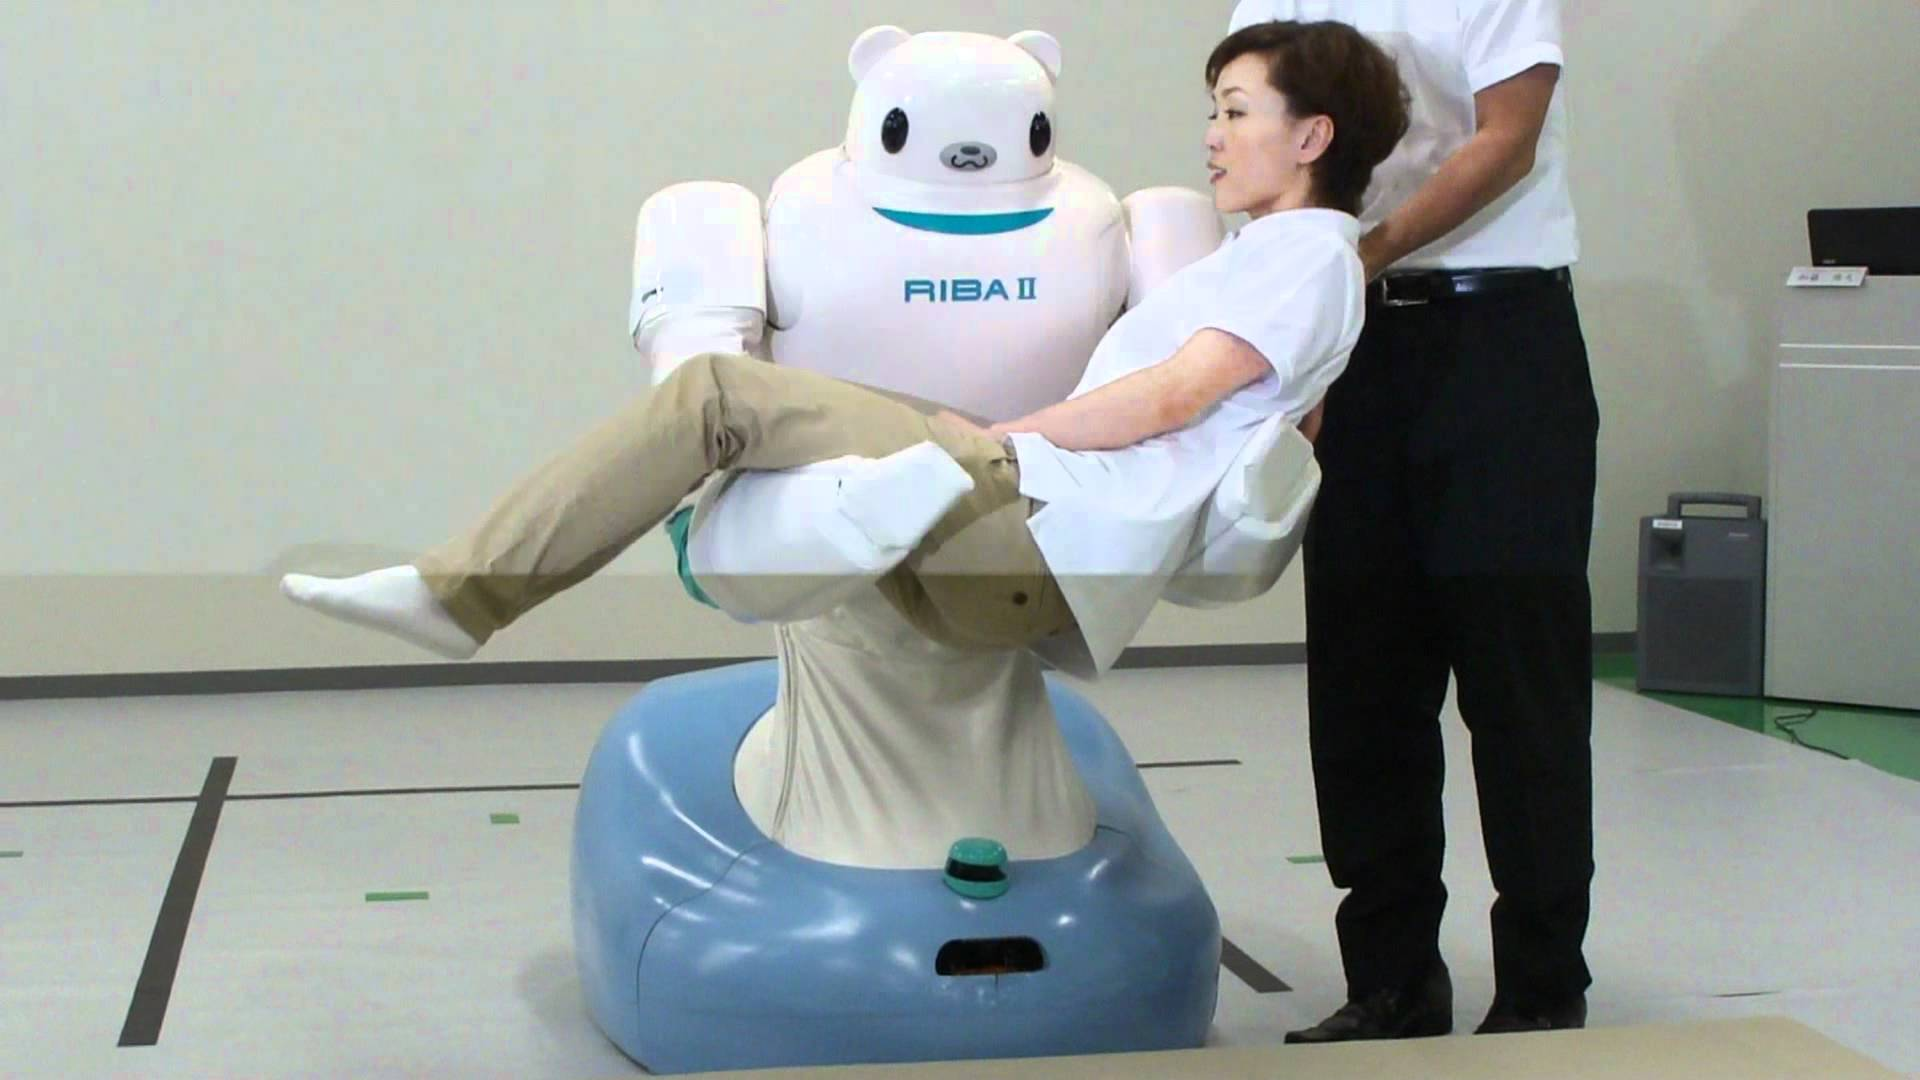
\includegraphics[scale=0.2]{images/StateOfArt/riba.jpg}
			\caption{RIBA II carrying a patient}
			\label{riba}
	\end{figure}
	\bigskip
\newpage



%\part{Proposed Solution} 
%Components
\section{Project components}
%%%%%%%%%% 3D PRINTER %%%%%%%%%%%%%%%%%%%%%%%%%%%%%%%%%%%%%%%%%%%%%%%%%%%%%
\subsection{3D Printer}

	3D printers are Computer Numerical Control (CNC) machines that are capable of transforming virtual 3D models created with a Computer Aided Design (CAD) software into real-world objects.\\

	Created in 1984 by Chuck Hull of 3D Systems Corp this technology was little-known to the general public and was mainly used in industries for short runs of difficult pieces.\\
	In 2005 Dr. Adrian Bowyer, from the University of Bath, UK, started the RepRap project. Its goal was "to produce a pure self-replicating device not for its own sake, but rather to put in the hands of individuals anywhere on the planet, for a minimal outlay of capital, a desktop manufacturing system that would enable the individual to manufacture many of the artifacts used in everyday life" \\

	Today a vast range of 3D printers co-exist, varying in size, price and materials used. \\


	$\rightarrow$ [RepRap, Zcorp, chocolate, liquid sint, micro, house building]\\

	$\rightarrow$ [table with different methods?]\\

	In this theses a RepRap Prusa Air 2 designed by Manuel Palacios is used. It is of a "fused filament fabrication additive manufacturing" type. This type of printers extrude mainly ABS or PLA plastics, and deposit new liquified material over ther previous layer, now solid, effectively building parts from the bottom up layer by layer.

	$\rightarrow$ \textbf {Terminal Imprusión Autorreplicante (T.I.A) }
	(add info + pic)
	Built within the scope of the Clone Wars project



%%%%%%%%%% 3D SOFTWARE %%%%%%%%%%%%%%%%%%%%%%%%%%%%%%%%%%%%%%%%%%%%%%%%%%%%
\subsection{Software}
	3D printers work by turning 3D models into plastic parts. These models are first modelled in a CAD program and then processed with a \textit{slicing} software to divide the model into layers of G-code, which is the standard language interpreted by CNCs. This is then introduced in a third piece of software which feeds it to the printer.

		\subsubsection{3D Modelling }
		In this project Sketchup has been used to create the printed parts. Owned by the company Trimble Navigation it is a WYSIWYG (What You See Is What You Get) modelling editor with a large online warehouse of parts available for download. \\

			\begin{figure}[H]
				\centering
				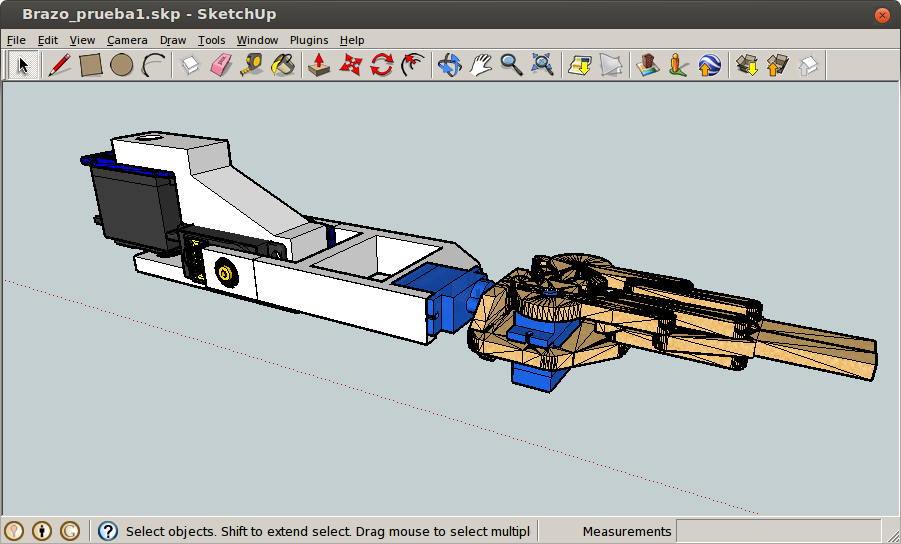
\includegraphics[scale=0.4]{images/ProjectComponents/sketchup-arm.png}
				\caption{SketchUp software}
				\label{}
			\end{figure}
			\bigskip

		In order to make it compatible with the slicing sofware, Sketchup's propietary format, \textit{SKP}, has to be converted to the standard \textit{STL}. In order to accomplish this the \textit{Su2stl.rb} plugin is installed. A new \textit{Plugins} menu appears in Sketchup which contains the Import/Export options, where the desired output format and model units are specified.



		\subsubsection{G-Code Generator} 
		Once the model is converted to \textit{STL} it then has to be sliced. Since 3D printers work by building layer upon layer of plastic, the model has to be transformed into the same format. The G-code generator converts the CAD model into layers of CNC instructions. There are three main slicing programs, each with their own benefits:

			\begin{itemize}
			  
			  \item Skeinforge: \hfill \\
			  The first slicing program used in homemade 3D printers. It is by far the most complete of the three. It allows the user to control each and every imaginable setting of the printer, from the axis' speeds to the retraction distance of the plastic into the extruder while moving. However, because of this it has a very steep learning curve which makes it unsuitable for the average consumer.

			  \item Slic3r:  \hfill \\
			  Slic3r was created as an user-friendly software, which only gives the final user a choice in the basic settings, such as printing speeds, filament widths or part infills. As a result it is an easier program to slice parts with a sufficient level of customization. It has nonetheless problems converting models with imperfections or broken shapes.
			  
			  \item Cura \hfill \\
			  Finally, Cura is also designed with user-friendliness in mind. This slicer is more robust than Slic3r, in that it will accept models with imperfections, and will try to correct them. It also features a box simulating the print area in which the model can be moved around, turned or scaled before printing.
			  This last feature is specially useful if minor changes need to be made, without returning to the CAD software.
			
			\end{itemize}



		\subsubsection{CNC Controller}


%%%%%%%%%%%% BATTERY %%%%%%%%%%%%%%%%%%%%%%%%%%%%%%%%%%%%%%%%%%%%%%%%%%%%%%
\subsection{Li-Ion Battery}

	The whole system is powered by a lithium ion 12V 6800mAh battery. 

		\begin{figure}[H]
				\centering
				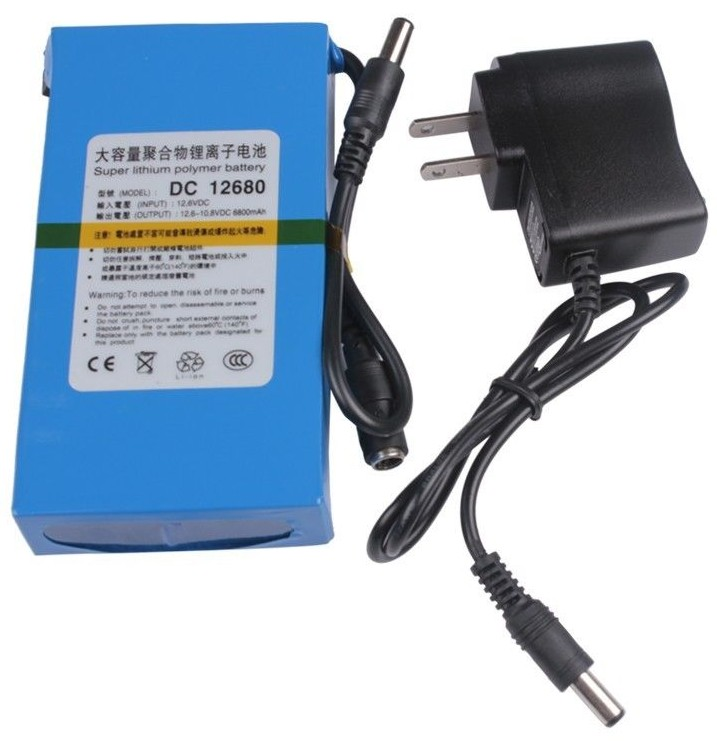
\includegraphics[scale=0.25]{images/ProjectComponents/battery.jpg}
				\caption{Li-ion 12V 6800mAh battery with charger}
				\label{}
		\end{figure}
		\bigskip

		\begin{figure}[H]
				\centering
				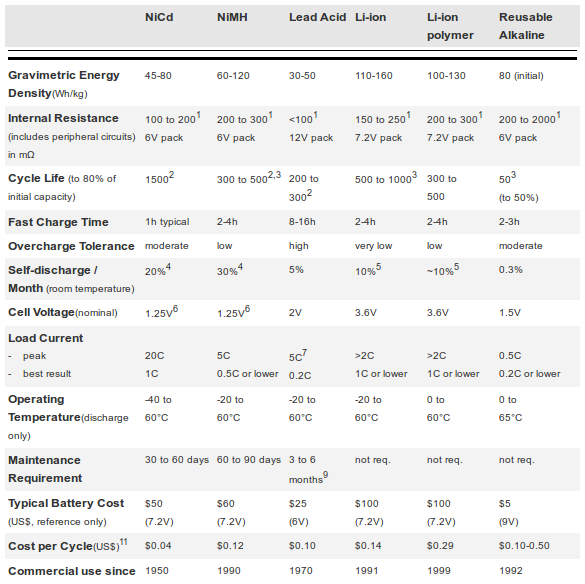
\includegraphics[scale=0.75]{images/ProjectComponents/battery-differences.png}
				\caption{Table comparing different battery technologies}
				\label{}
		\end{figure}
		\bigskip

%%%%%%%%%%% CONVERTER %%%%%%%%%%%%%%%%%%%%%%%%%%%%%%%%%%%%%%%%%%%%%%%%%%%%%
\newpage
\subsection{Voltage level converters}	
	
	\subsubsection{DC-DC Step-Down Converter}

		This DC-DC voltage conveter is used to decrease the battery's voltage from 12V to the 5V required by the logic components as well as the servomotors.

			\begin{figure}[H]
					\centering
					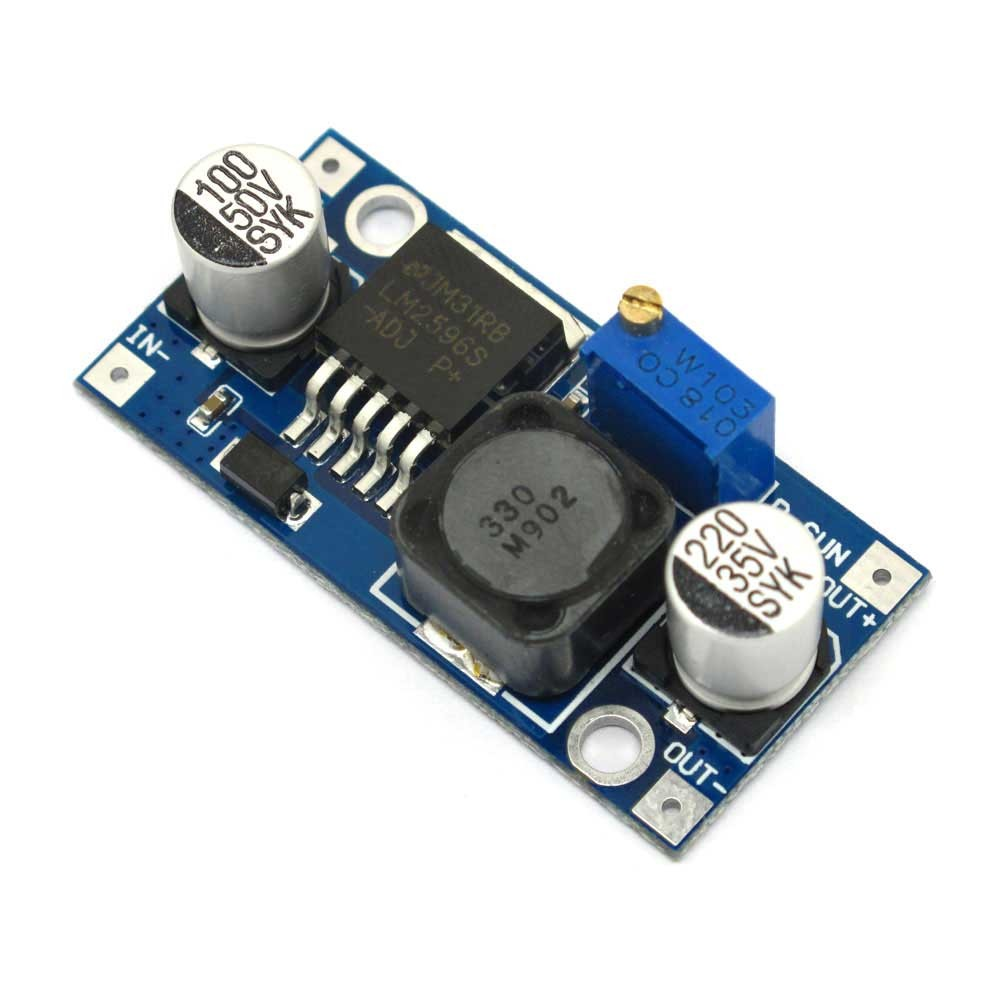
\includegraphics[scale=0.2]{images/ProjectComponents/buck.jpg}
					\caption{Step-down converter }
					\label{}
			\end{figure}
			\bigskip

		The converter's electrical specifications are:
			\begin{itemize}
				\item Adjustable input voltage: 3.2 - 40V
				\item Adjustable output voltage: 1.25 - 35V (require input voltage 1.5V high than output voltage)
				\item Max. output current: 3A
			\end{itemize}

	\subsubsection{Bi-directional logic level converter}

		This logic level converter is used to enable serial communication between the Arduino and the Raspberry Pi, since the latter's 3.3V operation point could be damaged by the former's 5V high-level. 

			\begin{figure}[H]
					\centering
					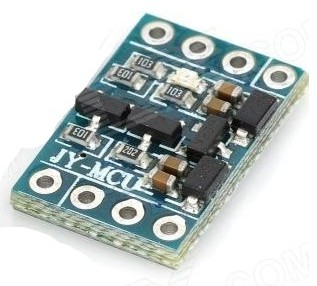
\includegraphics[scale=0.4]{images/ProjectComponents/logic-voltage.jpg}
					\caption{Bi-directional logic level converter }
					\label{}
			\end{figure}
			\bigskip

		This board is used with UART communication, but is equally adequate for I$^2$C, SPI or even one-wire communication.
 
%%%%%%%%%%% DC MOTORS %%%%%%%%%%%%%%%%%%%%%%%%%%%%%%%%%%%%%%%%%%%%%%%%%%%%%
\subsection{Motors}

	\subsubsection{GA25Y370 DC motor}
	
		\begin{figure}[H]
			\centering
			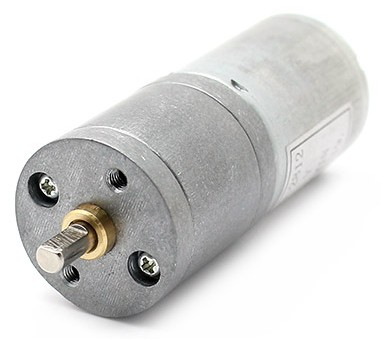
\includegraphics[scale=0.4]{images/ProjectComponents/motor.jpg}
			\caption{GA25Y370 motor }
			\label{}
	\end{figure}
	\bigskip

	\subsubsection{GOTECK GS-551MG servomotor}

		\begin{figure}[H]
			\centering
			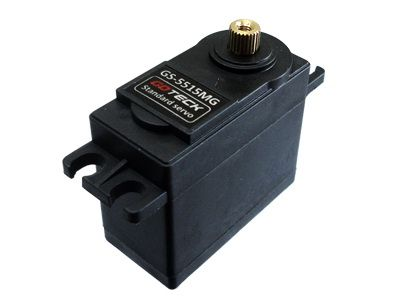
\includegraphics[scale=0.5]{images/ProjectComponents/servo1.jpg}
			\caption{GOTECK GS-551MG servo }
			\label{}
	\end{figure}
	\bigskip


	\subsubsection{TowerPro SG90 servomotor}

		\begin{figure}[H]
			\centering
			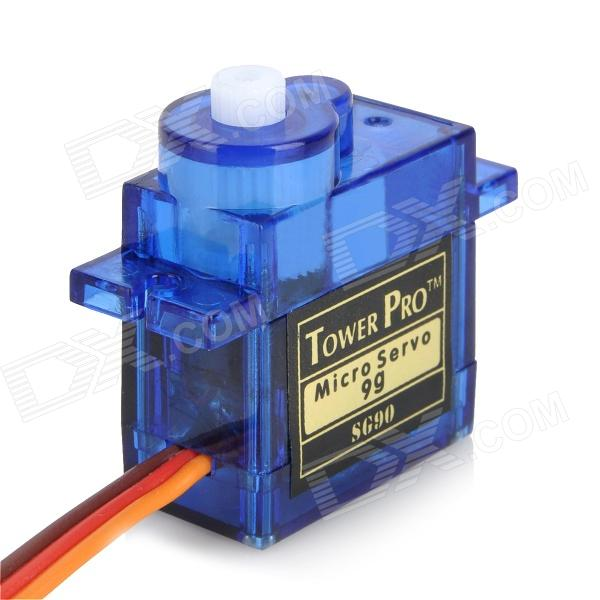
\includegraphics[scale=0.25]{images/ProjectComponents/servo2.jpg}
			\caption{TowerPro SG90 servo }
			\label{}
	\end{figure}
	\bigskip





%%%%%%%%%%%% ARDUINO %%%%%%%%%%%%%%%%%%%%%%%%%%%%%%%%%%%%%%%%%%%%%%%%%%%%%%
\newpage
\subsection{Arduino}

	Arduino is a family of low-cost electronic boards designed to be easily programmable. From the official Arduino website, "Arduino is an open-source electronics prototyping platform based on flexible, easy-to-use hardware and software. "\\

	Arduino is programmed using its own language, which is merely a set of C/C++ functions compiled with \textit{avr-g++}. They can nonetheless be programmed in pure C or C++ in an external IDE and have code uploaded as any other AVR board.\\

	In this proyect an Arduino Nano v3 with an ATmega 328 microcontroller has been chosen mainly due to its processing power and reduced size.
		
		\begin{figure}[H]
			\centering
			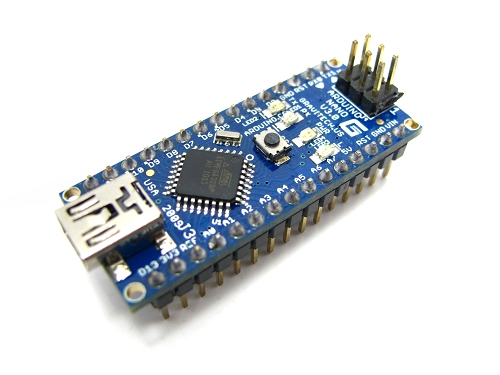
\includegraphics[scale=0.4]{images/ProjectComponents/arduino.jpg}
			\caption{Arduino Nano v3 }
			\label{}
		\end{figure}
		\bigskip

	The official Arduino Nano V3 specifications are:
		\begin{itemize}
			\item \textbf{Microcontroller:} Atmel ATmega168 or ATmega 328
			\item \textbf{Operating Voltage (logic level):} 5V
			\item \textbf{Input Voltage (recommended):} 7-12V
			\item \textbf{Input Voltage (limits):} 6-20V
			\item \textbf{Digital I/O Pins:} 14 (of which 6 provide PWM output)
			\item \textbf{Analog Input Pins:} 8
			\item \textbf{DC Current per I/O Pin:} 40mA
			\item \textbf{Flash Memory:} 16 KB (ATmega168) or 32 KB (ATmega328), of which 2 KB used by bootloader
			\item \textbf{SRAM:} 1 KB (ATmega168) or 2 KB (ATmega328)
			\item \textbf{EEPROM:} 512 bytes (ATmega168) or 1 KB (ATmega328)
			\item \textbf{Clock Speed:} 16MHz
			\item \textbf{Dimensions:} 0.73'' x 1.70''
			\item \textbf{Communications:} UART, SPI and I$^2$C buses
		\end{itemize}



%%%%%%%%%%% RASPBERRY %%%%%%%%%%%%%%%%%%%%%%%%%%%%%%%%%%%%%%%%%%%%%%%%%%%%%
\newpage
\subsection{Raspberry Pi}

	From the official website of the homonymous foundation, the Raspberry Pi is a "credit-card sized computer that plugs into your TV and a keyboard. It is a capable little computer which can be used in electronics projects."\\

		\begin{figure}[H]
				\centering
				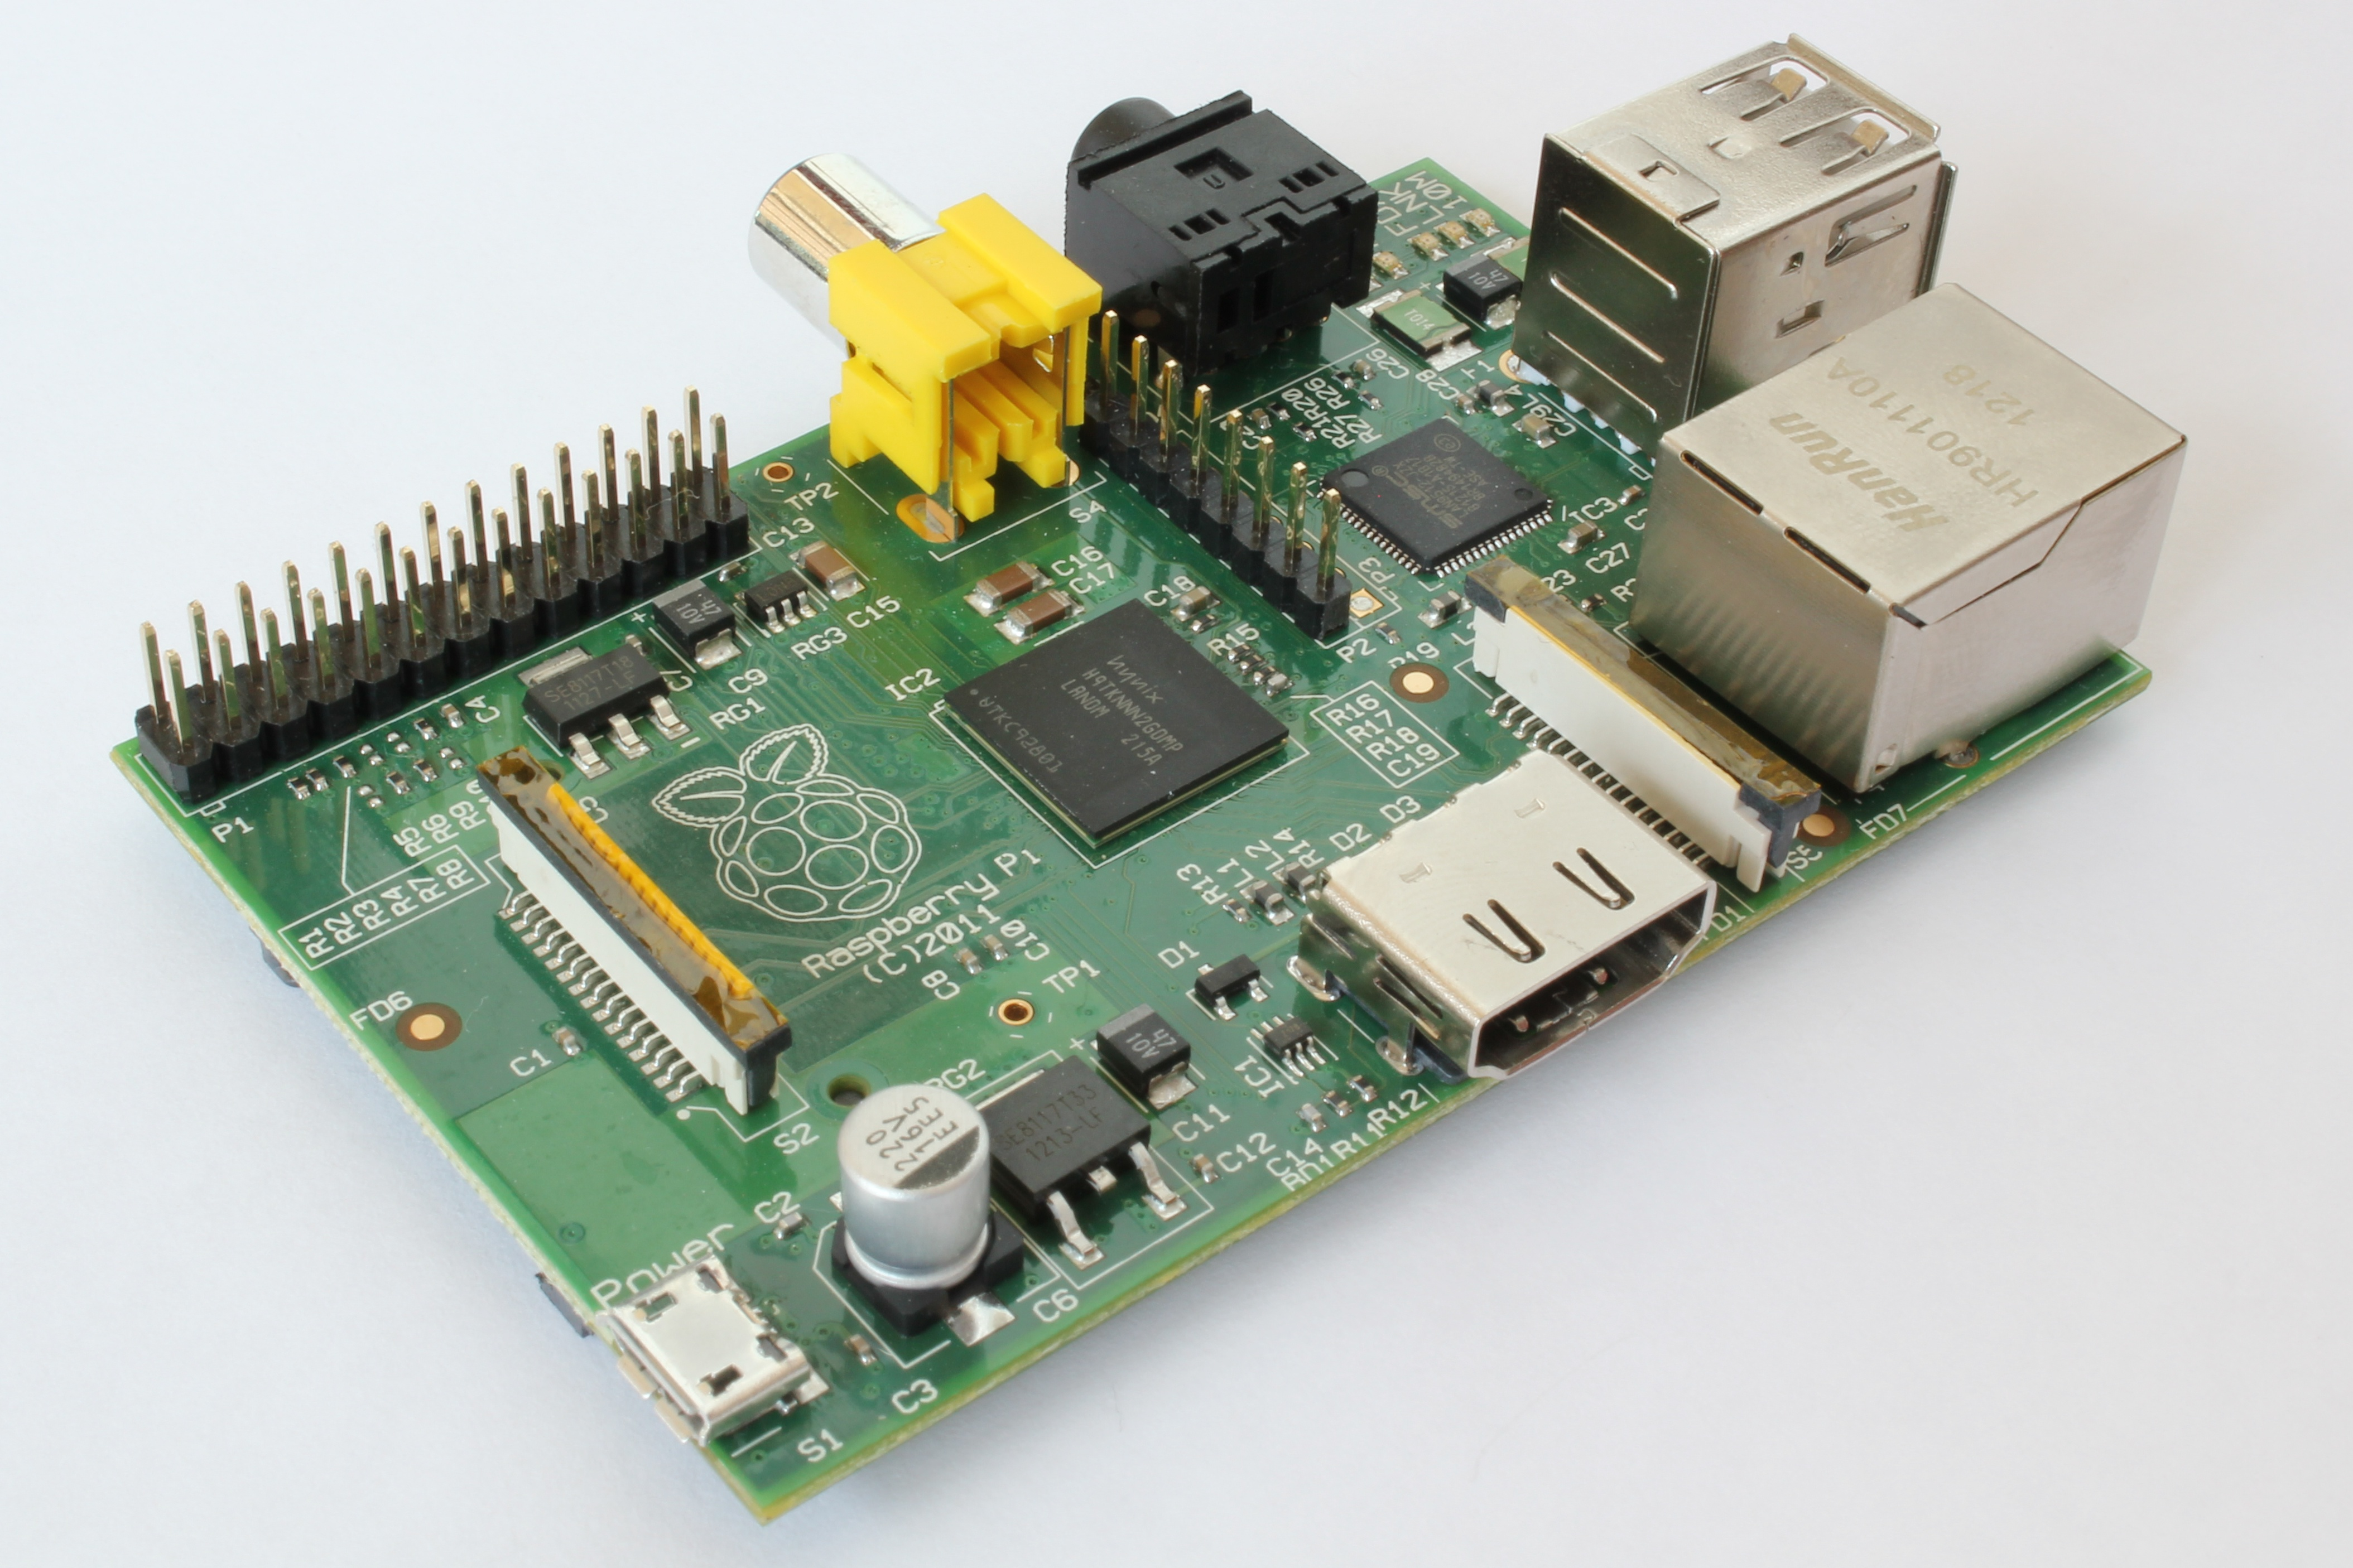
\includegraphics[scale=0.07]{images/ProjectComponents/raspberry.jpg}
				\caption{Raspberry Pi model B}
				\label{}
		\end{figure}
		\bigskip

	Available in two models, A and B, the Raspberry has a Broadcom BCM2835 System On a Chip, which includes an ARM1176JZF-S 700MHz processor and a VideoCore IV GPU. It includes as well a 256Mb RAM, upgraded to 512Mb in model B.\\

	\bigskip

	The Pi features: 
		\begin{itemize}
			  \item HDMI, composite and raw DSI video outputs
			  \item 3.5mm audio jack
			  \item SD card socket
			  \item Low-level peripheral connections including:
			  	\begin{itemize}
			  	\item 8 General Purpose Input Output (GPIO) pins
			  	\item Universal Asynchronous Receiver Transmitter (UART) bus
			  	\item Inter-Integrated Circuit (I$^2$C) bus
			  	\item 2 Serial Peripheral Interface (SPI) buses
			  	\item Power pins: 3.3V, 5V and GND
			  	\end{itemize}
			  \item Ethernet socket
			  \item USB hub (1 socket in model A, 2 in model B)

		\end{itemize}

	The main storage unit is the SD card, and that is where the OS is flashed, normally a Linux distribution. The most popular is Raspbian, an adapted version of Debian Wheezy, although other Linux distros or even other OS like Android or XBMC can be used.

		\begin{figure}[H]
		    \centering
		    \begin{subfigure}[b]{0.3\textwidth}
		        \centering
		        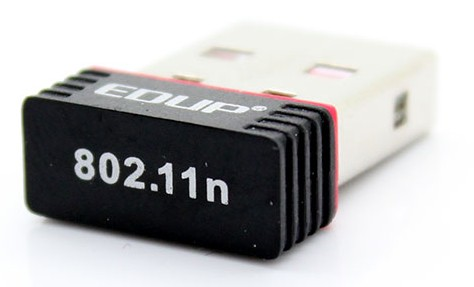
\includegraphics[scale=0.25]{images/ProjectComponents/wifi.jpg}
				\caption{WiFi USB dongle}
		        \label{}
		    \end{subfigure}
		    \hfill
		    \begin{subfigure}[b]{0.3\textwidth}
		        \centering
		        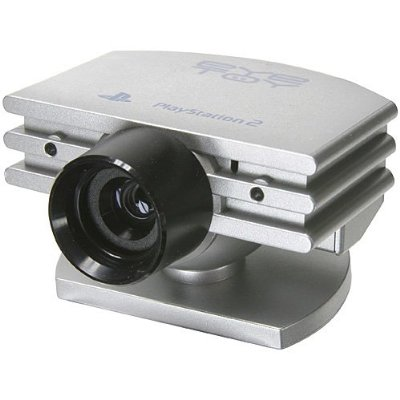
\includegraphics[scale=0.25]{images/ProjectComponents/camera.jpg}
				\caption{PlayStation 2 EyeToy }
		        \label{}
		    \end{subfigure}
		    \hfill
		    \begin{subfigure}[b]{0.3\textwidth}
		        \centering
		      	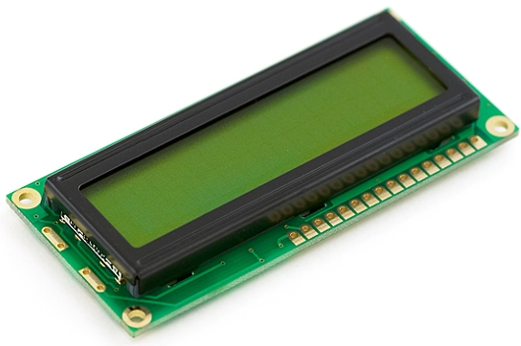
\includegraphics[scale=0.25]{images/ProjectComponents/lcd.jpg}
				\caption{LCD screen 16x2}
		        \label{}
		    \end{subfigure}
		    \caption{Raspberry Pi peripherals}
		    \label{}
		\end{figure}


	In this proyect a Raspberry Pi model B running Raspbian manages the software side of the robot. It has an EDUP 802.11n WiFi USB dongle , a PlayStation 2 EyeToy USB camera and a 16x2 character LCD screen connected in order to create a WIFI Access Point, stream video to the user and signal its status respectively.



% %%%%%%%%%%% LCD SCREEN %%%%%%%%%%%%%%%%%%%%%%%%%%%%%%%%%%%%%%%%%%%%%%%%%%%%
% \subsection{LCD Screen}

% 	\begin{figure}[H]
% 			\centering
% 			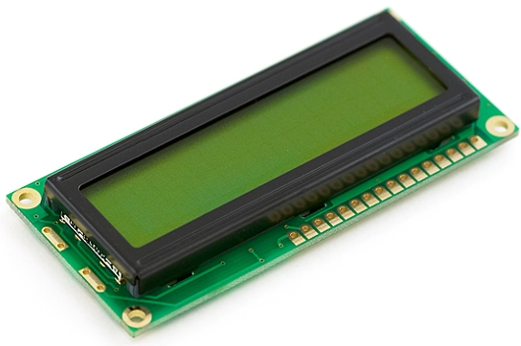
\includegraphics[scale=0.4]{images/ProjectComponents/lcd.jpg}
% 			\caption{LCD screen 16x2}
% 			\label{}
% 	\end{figure}
% 	\bigskip

% %%%%%%%%%%% WIFI USB %%%%%%%%%%%%%%%%%%%%%%%%%%%%%%%%%%%%%%%%%%%%%%%%%%%%%%
% \subsection{WiFi USB}

% 	\begin{figure}[H]
% 			\centering
% 			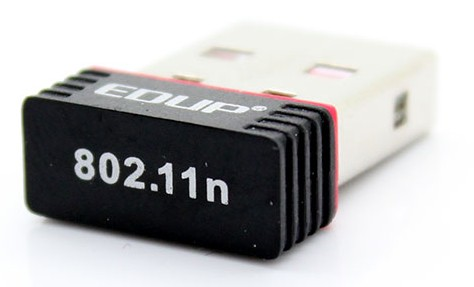
\includegraphics[scale=0.4]{images/ProjectComponents/wifi.jpg}
% 			\caption{WiFi USB dongle}
% 			\label{}
% 	\end{figure}
% 	\bigskip

% %%%%%%%%%%% CAMERA %%%%%%%%%%%%%%%%%%%%%%%%%%%%%%%%%%%%%%%%%%%%%%%%%%%%%%%%
% \subsection{Camera}

% 	\begin{figure}[H]
% 			\centering
% 			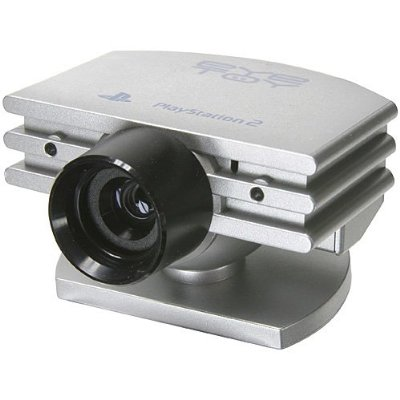
\includegraphics[scale=0.4]{images/ProjectComponents/camera.jpg}
% 			\caption{PlayStation 2 EyeToy camera }
% 			\label{}
% 	\end{figure}
% 	\bigskip






%%%%%%%%%%% ANDROID %%%%%%%%%%%%%%%%%%%%%%%%%%%%%%%%%%%%%%%%%%%%%%%%%%%%%%%
\newpage
\subsection{Android Phone}

	\begin{figure}[H]
			\centering
			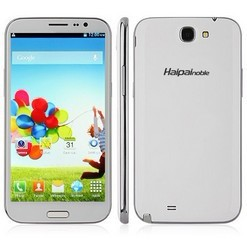
\includegraphics[scale=0.8]{images/ProjectComponents/android.jpg}
			\caption{Android smartphone Haipai Noble H868}
			\label{}
	\end{figure}
	\bigskip


\newpage
%Components
\section{Design alternatives}
Before arriving to its final form, several designs for the PD-SD were considered. Here are listed the various alternatives weighed:

\paragraph{Humanoid} The most natural form an assitive robot can take to replace a person in home chores is that of another, since homes are designed to be controlled and navigated by humans. \\

Therefore a humanoid robot was the inmediate answer: its degrees of freedom would enable it to carry out the same tasks as their human counterparts, it would have the right size to be able to handle objects placed in high furniture and it would have a form that would generate an emotional response from the user.\\

However, the humanoid has one major disadvantage, control. While two-legged robots do exist, as seen previously with Honda's ASIMO, they are very unstable and require active control algorithims to balance it. \\

To make the droid stable even when unpowered and to simplify the algorithims the legs were replaced by a wheeled base. This also had the side effect of reducing the cost, since each wheel would be driven by one motor to provide a differential drive, instead of a total of twelve motors for a pair of full human like legs, with three to simulate the hip joint, one for the knee and two more for the ankle, per leg.\\


\paragraph{Four wheels} The first wheeled base design envisaged four wheels in order to keep it stable, each with its own motor. However, the design is redundant, as a two-wheeled base with a caster at the rear end is equally stable but reduces the number of active wheels. This decreases the price, the power consumption, frees up two pins on the micro controller and reduces the length of the code, while remaining suitable to support the robot.


\paragraph{Exoskeleton} One of the first designs is shown in Figure \ref{exoskeleton}. It featured a robot with an exoskeleton and a central beam. This version granted different levels into which the various components could be placed while hiding the cables inside. \\

	\begin{figure}[H]
			\centering
			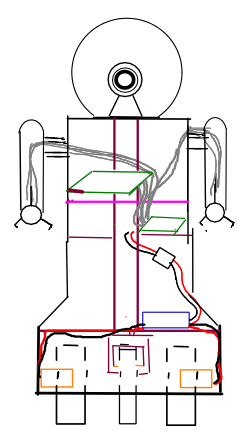
\includegraphics[scale=0.4]{images/Diagrams/exoskeleton}
			\caption{First sketch of the PD-SD}
			\label{exoskeleton}
	\end{figure}
	\bigskip

However, it provided very little stability and a design with a more human-like skeleton was chosen.\\


\paragraph{Arm designs} The most natural configuration for the robot to grasp objects would be that of a human hand, especially taking into account that most objects are designed to be handled it.\\

However, in the final design a parallel gripper was chosen because it reduced the number of motors needed to one per gripper, while having two parallel-closing fingers capable of gripping objects of differing sizes.\\

The first CAD model of the arm is shown in Figure \ref{firstArm}. It included five motors, four directional and one to control the gripping action. The orientation of the servomotors ensured rotation in all three axes, with two degrees of freedom in the pitch angle. This is done to give the possibility of linear movement useful for lifting and lowering objects in cluttered spaces.  
\\	

	\begin{figure}[H]
			\centering
			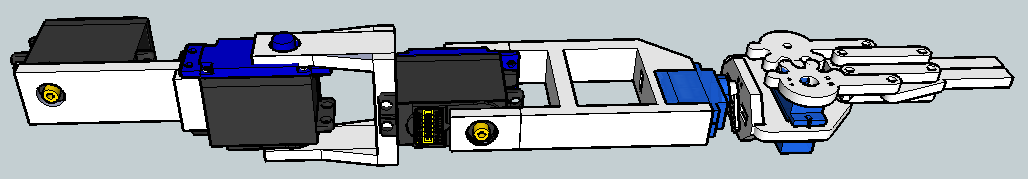
\includegraphics[scale=0.4]{images/Diagrams/firstArm}
			\caption{First design of the arm}
			\label{firstArm}
	\end{figure}
	\bigskip

In Figure \ref{finalArm} the final design is shown. While it keeps the original servo orientation, the placement is modified to reduce the distance between the two leftmost motors and so reduce the torque needed to lift objects. \\
The plastic parts have also been modified to enclose the motors, which now are firmly secured in place, and to support the weight of the arm instead of relying in the screws to do so.

	\begin{figure}[H]
			\centering
			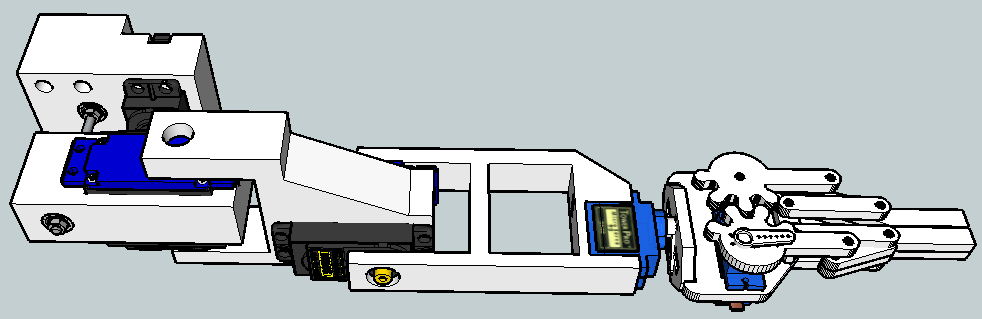
\includegraphics[scale=0.4]{images/Diagrams/finalArm}
			\caption{Final design of the arm}
			\label{finalArm}
	\end{figure}
	\bigskip


\newpage
%Assembly-HW
\section{Hardware assembly}
%\section{Personal Domestic Service Droid}
%%%%%%%%%% MECHANIC %%%%%%%%%%%%%%%%%%%%%%%%%%%%%%%%%%%%%%%%%%%%%%%%%%%%%%%
\subsection{Mechanical structure}
\subsubsection{Upper body}
denavit hartenberg for arms

\subsubsection{Lower body}
election of wheels vs legs

\subsubsection{Assembly}
cad models of assembly

list of all the parts with images
images with assembly 

diagram of complete assembly with servo+motor letters assigned















\subsection{Connections}

This section will present how the different elements composing the robot are connected, first from the electrical point of view, then from a means of communication angle and finally from the different programs' interactions perspective.



%%%%%%%%%% ELECTRIC %%%%%%%%%%%%%%%%%%%%%%%%%%%%%%%%%%%%%%%%%%%%%%%%%%%%%%%

\subsubsection{Electrical connections}

Figure \ref{electricDiagram} shows how the different electric and electronic components are interconnected.  As it can be seen, different voltage levels co-exist within the robot, so regulators are placed to ensure the components function correctly. \\

The DC motors need the highest voltage to work, and so are connected to the battery, which provides them with the 12V they need. However they have to be controlled by the Arduino, hence the need for a driver that will turn on and off the 12V rails from 5V signals.\\

The rest of the components operate at 5V, which is why the step-down converter is used to convert the battery's 12V output into the desired level. The Raspberry Pi, Arduino and servomotors are connected to this rail.\\

Finally, the Raspberry communicates with the Arduino through the former's UART pins, which operate at a 3.3V level and can be damaged by the latter's 5V level pins. To avoid this a logic level shifter is introduced, which ensures data transmission without compromising the hardware's integrity.\\

	\begin{figure}[H]
			\centering
			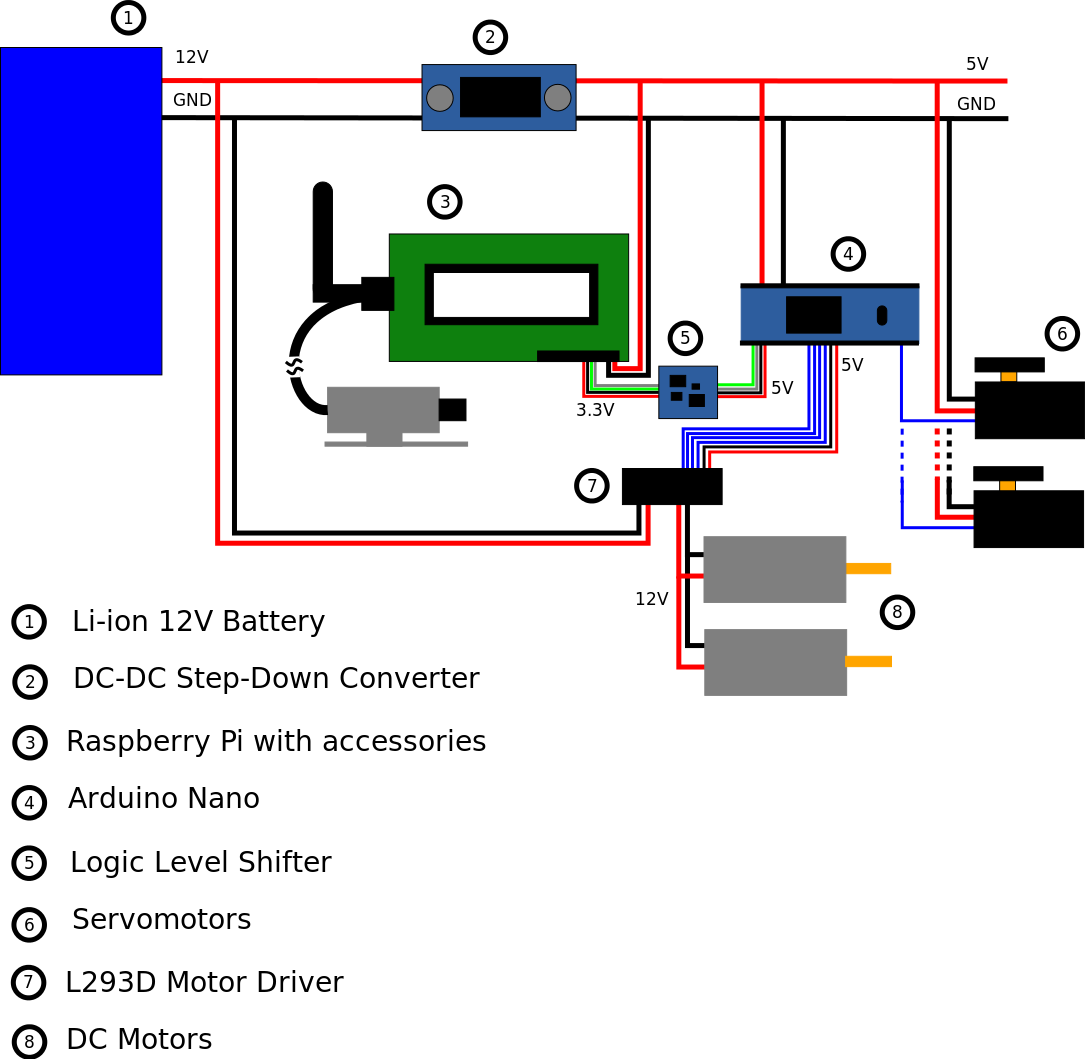
\includegraphics[width=15cm, angle=0]{images/Diagrams/electrical.png}
			\caption{Electrical connections diagram }
			\label{electricDiagram}
	\end{figure}
	\bigskip
	
\bigskip


The previous diagram shows how all components are interconnected, but to increase its clarity some connections have not been shown in detail. The following diagrams show how the remaining elements are wired pin by pin.

	\begin{itemize}
	\item Figure \ref{gpioDetail} shows the conections between the LCD and Rasbperry Pi and the Raspberry, Arduino and the logic voltage shifter pins.
	\end{itemize}

	\begin{figure}[H]
			\centering
			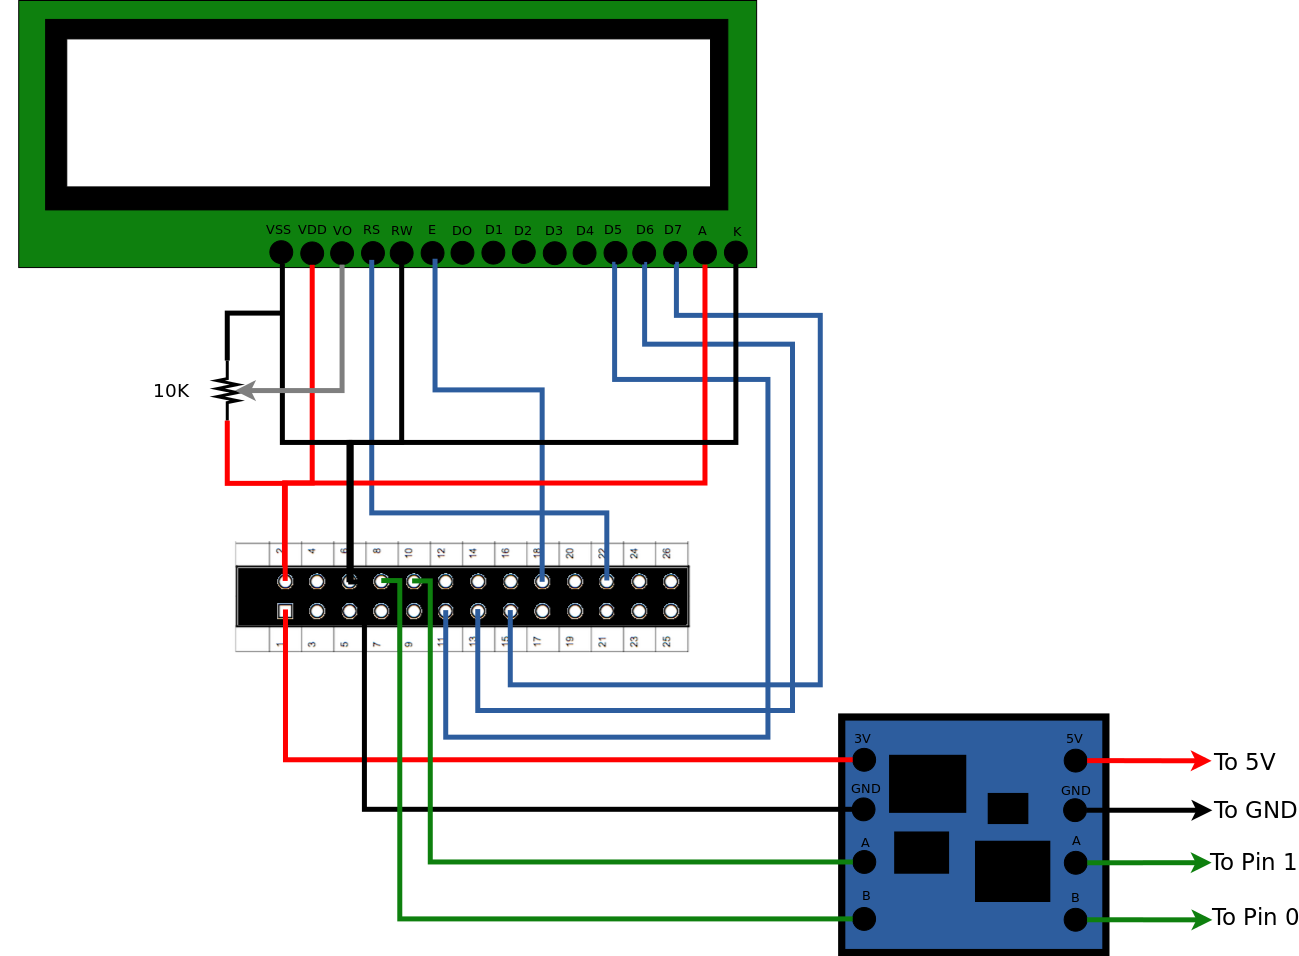
\includegraphics[width=15cm, angle=0]{images/Diagrams/detail.png}
			\caption{Detail of LCD and Serial connections }
			\label{gpioDetail}
	\end{figure}
	\bigskip


	\bigskip
	\begin{itemize}
	\item Figure \ref{hbridgeDetail} shows the wiring between the motor driver, the motors and the Arduino.
	\end{itemize}
	
	\begin{figure}[H]
			\centering
			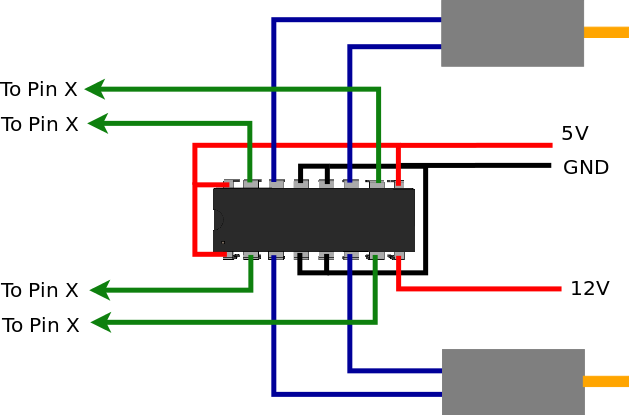
\includegraphics[scale=0.5, angle=0]{images/Diagrams/hbridge.png}
			\caption{Detail of motor driver wiring }
			\label{hbridgeDetail}
	\end{figure}
	\bigskip

	\begin{itemize}
	\item Figure X shows which element is connected to each of the Arduino pins

	\item "table with servo +motor letters assigned to arduino pins"
	\end{itemize}


%%%%%%%%%% LOGIC %%%%%%%%%%%%%%%%%%%%%%%%%%%%%%%%%%%%%%%%%%%%%%%%%%%%%%%

\subsubsection{Logic connections}

Figure \ref{logicDiagram} shows how the different components communicate between themselves. As it can be seen, the user controls the robot from the Android application. This implements a bidirectional communication over wifi with the Raspberry Pi, which is used to both send the Raspberry data concerning the movement of the different motors and to receive the video stream from the robot's onboard camera. The Raspberry then communicates over Serial port with the Arduino, which takes care of the data received to obey the user's commands.\\

	\begin{figure}[H]
			\centering
			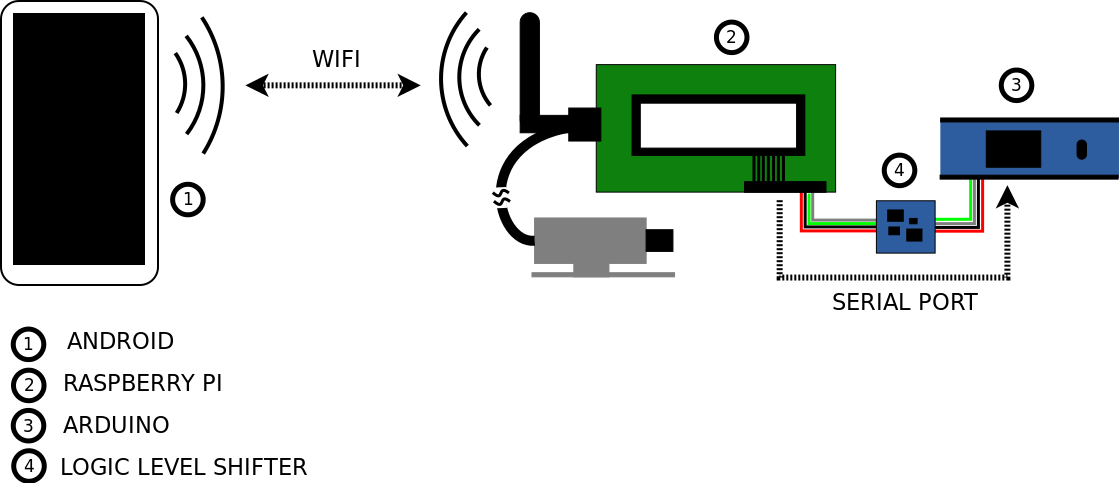
\includegraphics[width=15cm, angle=0]{images/Diagrams/logic.png}
			\caption{Logic connections diagram }
			\label{logicDiagram}
	\end{figure}
	\bigskip

%%%%%%%%%% SW %%%%%%%%%%%%%%%%%%%%%%%%%%%%%%%%%%%%%%%%%%%%%%%%%%%%%%%

\subsubsection{Software connections}

Figure \ref{swDiagram} shows how the different programs interconnect the various components. It can thus be seen that the Raspberry Pi will first create a wifi network and then start to stream video through it. The android phone on the other hand will connect itself to the recently created network and will use it to emit the commands given by the user. The Raspberry will have already started the IP/UART Bridge, and will send the data received from the phone to the Arduino. Finally, the latter will execute its code to execute the orders received.\\

	\begin{figure}[H]
			\centering
			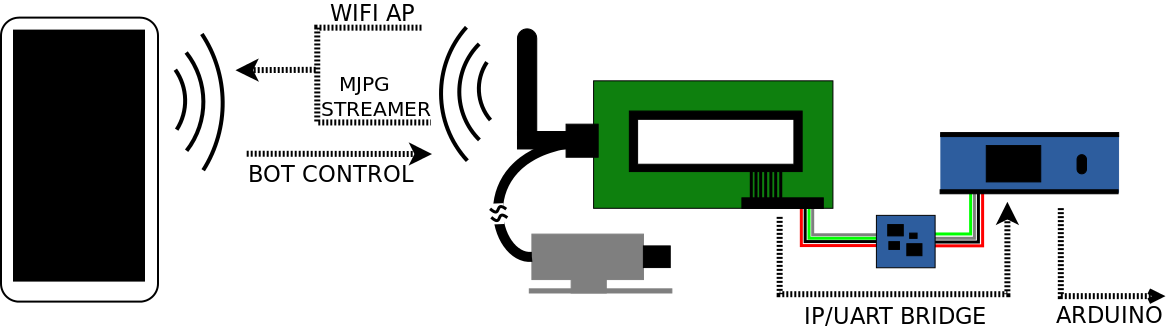
\includegraphics[width=15cm, angle=0]{images/Diagrams/software.png}
			\caption{Software connections diagram }
			\label{swDiagram}
	\end{figure}
	\bigskip


\newpage
%Arduino
\section{Arduino}
\subsection{Overview}
Arduino refers both to the microcontroller board used to interface with sensors and actuators and to the software used to program it.\\

As a microcontroller, an Arduino is a relatively cheap development board useful for controlling many input and output pins, either digital or analog, in a single board solution that plugs directly into the computer over USB.\\

As a software environment, it provides a simple IDE with many code examples, a bootloader to program microcontroller chips directly with almost no external components and a growing user community that creates libraries for different sensors and communication protocols among others.\\

All Arduino programs follow the structure presented in Figure \ref{arduinoSkeleton}, namely one Setup function and one Loop function. The first is executed only once at the beginning of the program, while the latter is equivalent to a "while(1)" block, meaning that any code entered into it will be repeated until the microcontroller shuts down or is reset.\\

\begin{figure}[H]
      \centering
      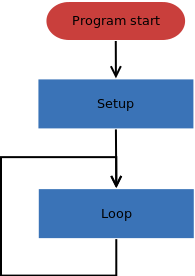
\includegraphics[scale=.8]{images/Diagrams/arduinoSkeleton.png}
      \caption{Arduino code skeleton }
      \label{arduinoSkeleton}
\end{figure}
\bigskip



%%%%%%%%%% FLOWCHART%%%%%%%%%%%%%%%%%%%%%%%%%%%%%%%%%%%%%%%%%%%%%%%%%%%%%%%
\newpage
\subsection{Code}

In this section the code written for the robot's controller will be explained. A flowchart diagram of the program is illustrated by Figure \ref{arduinoFlowchart}.\\

	\begin{itemize}
        
	    \item As it can be seen, the Arduino first defines all the robot's data, including the motor, servomotor and communication pins. This ensures the microcontroller knows where to send each datum once the user connects to the robot.\\

		\item The program then enters its Loop function. Here it will check if the serial port is available, eg the user has sent a stream of data. Once the port is available, the Read function is called, which stores every byte received into a string to be used later. Once the reading has ended the code checks if it has received a special end-of-line character that signals the end of the data stream. If all the data was retrieved the code moves on to the next function.\\

		\item The Parse function is called upon next. This function's purpose is to break and convert the previously stored string into the corresponding variables needed by each element, taking into account their sizes and types. Hence, it transforms one line of numbers into many parameters such as rotation angle, arm selection or movement direction which will be used by the next function.\\

		\item With the data correctly formatted, the program executes the Process function which is where the "thinking" is done. Here are defined all the rules the robot must follow, such as knowing which claw to close depending on the side chosen by the user but closing both if the symmetry box was checked. It takes the data provided by the previous function and processes them to end up with a structured list of variables ready to be assigned to each element.\\

		\item In the next step the Write function is called. This very simple function goes through the previous list assigning each variable to the corresponding element's assigned pins.\\

		\item Finally, the code clears the initial string to make space for new data, resets the flag informing of the correct retrieval from the serial port and proceeds to the next iteration within the Loop function, restarting the process.\\

	\end{itemize}

	\begin{figure}[H]
			\centering
			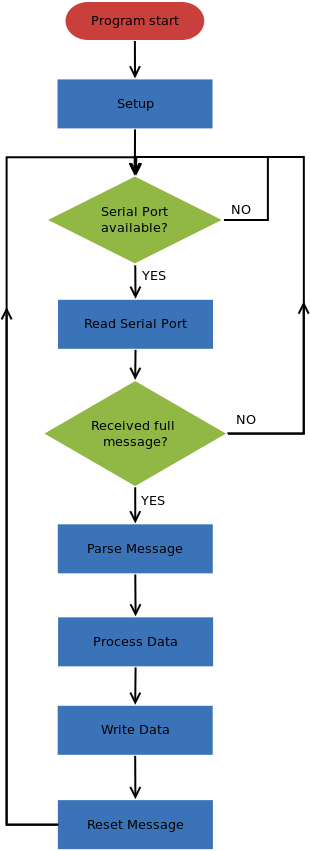
\includegraphics[scale=0.75]{images/Diagrams/arduino2.png}
			\caption{Arduino program flowchart }
			\label{arduinoFlowchart}
	\end{figure}
	\bigskip



\newpage
%Raspberry
\section{Raspberry Pi}
The Raspberry Pi carries out three main duties to ensure everything works correctly. These include creating a wireless connection, streaming images from the camera to the phone and transmitting the data received from the phone to the microcontroller.\\

 These are all placed into the \textit{/etc/rc.local} file so the system initializes them automatically each time the robot is turned on, with no need for human interaction.

\subsection{Wireless Communications}% WiFi Acces Point

The chosen means of communication between human and humanoid was wifi. This is so because it is a widely established technology, with great compatibility and in a great number of cases is already installed in the homes of users.\\

Three methods were considered: connection to an existing wifi network, creation of an Ad-Hoc connection and establishment of a wifi Access Point.

\subsubsection{Existing network:}

asdlkfasdjfasdofjkalsdz

\subsubsection{Ad-Hoc connection:}



\subsubsection{Wifi Access Point:}




\subsection{MJPG Streamer}




\subsection{IP/UART Bridge} 

\newpage
%Android
\section{Android} 
Android has been used instead of iphone or windows because ... marketshare, graphs, prices etc


app skeleton, typical app example, android studio etc


this app





\begin{figure}[H]
      \centering
      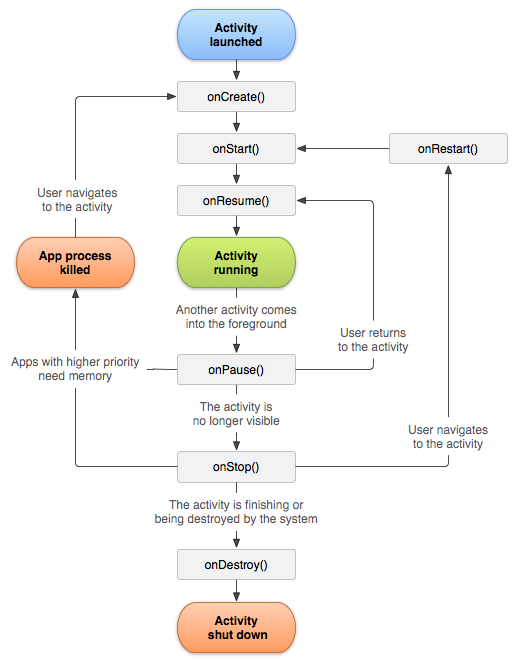
\includegraphics[scale=.8]{images/Diagrams/android_activity_lifecycle.png}
      \caption{Android app activity lifecycle }
      \label{androidActivity}
  \end{figure}
  \bigskip

\newpage


%FUTURE
%\part{Conclusion} 
\section{Conclusion}
\subsection{Objectives completition}
It can be said that the proyect \textit{Design, construction and programming of a low cost, Open Source robot for assistive activities} has accomplished the objectives originally set:

	\begin{itemize}

	\item Different configurations have been studied in order to achieve a working prototype

	\item The final design, derived from the previous study has been modelled using the CAD program SketchUp

	\item The modelled parts have been created by means of a 3D printer

	\item The parts have been assembled and the electronics installed in order to create a functioning robot

	\item The Arduino board has been programmed to control both the arms as the base following the user's commands

	\item The Raspberry Pi has been programmed to:

		\begin{itemize}
		
		\item set up a wifi network that enables bidirectional communication between the user and the PD-SD independently of pre-existing networks

		\item stream the video feed captured by the on-board camera to the user's phone

		\item receive the user's instructions and send them to the Arduino over serial communication while the socket connection maintained

		\item initialize a script when booting to do all the previous automatically

		\end{itemize}

	\item Program the Android application \textit{Bot Control} to allow the user to take control of the Droid while being able to monitor what it sees


	\end{itemize}



The robot is also low cost, as it can be seen in the ``Budget" annex and Open Source, as all of the code can be downloaded from this GitHub repository \footnote{https://github.com/alvaroferran/Proyecto}.\\

Finally, while it is a working prototype, it can be improved by implementing the suggestions found in the following section.





















\newpage
\subsection{Future work}

The PD-SD is a very versatile robot, but it is far from complete and many new features can be added. A few of them could be:

\paragraph{iOS application:} Although Android has the largest market share, iOS users are not negligeable, and the most immediate improvement would be to develop a version of Bot Control for that system, in order to increase the number potential users.

\paragraph{User routine programming:} Another interesting feature would be to include the ability for the non-technical user to program chores they want the robot to accomplish, such as bringing them a glass of water every morning or opening the blinds at a set hour. \\

This would give the users a higher quality service from their PD-SD, since they would be able to demand tasks as needed.



\paragraph{Enhanced gripper:}  The PD-SD currently features two parallel grippers, which enable it to grasp objects of different sizes due to the closing mechanism. However, complex figures may not be easy to hold to, and a vacuum gripper would be the ideal solution for this. By being pushed into the object while filled with air, the gripper adapts its shape to fit the object better, and when the air is removed the object remains firmly in place until it is released again. Figure \ref{gripper} illustrates this procedure.

	\begin{figure}[H]
			\centering
			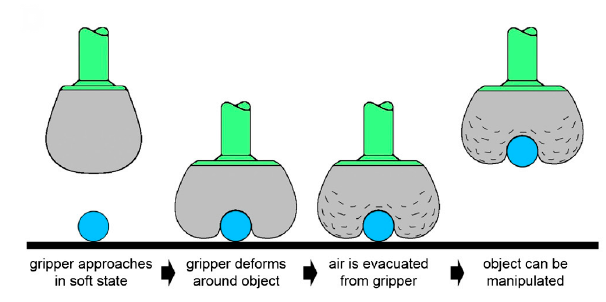
\includegraphics[scale=0.7]{images/Conclusion/gripper.png}
			\caption{Vacuum gripper  }
			\label{gripper}
	\end{figure}
	\bigskip


\paragraph{Full-size droid:} The final objective of this project is to eventually build a full-size robot capable of actually helping in the house by being able, for example, to reach into the higher cabinets of the kitchen or carry objects from one place to another.\\ 

In order to do this the robot must have a certain height and strength, so while the software would largely remain unchanged, the actuators and body parts would certainly need a revision. 


\paragraph{Computer vision:} Finally, adding computer vision capabilities to the robot would greatly enhance its capabilities. By integrating a library such as OpenCV, the robot could be able to recognize its charging dock by means of a symbol, or simply the phrase ``Charging dock", and could move towards it when the battery level descended.\\

Another feature would be to implement a pathfinding algorithim to take into account the walls, doors and floor of the house and make the robot navigate throughout it autonomously, for instance to fulfill one of the previously mentioned ``programmed chores".


\newpage
%BIBLIIOGRAPHY
\begin{thebibliography}{9}

\bibitem{automata-monk}
``The Monk Automaton of 1560" http://thehairpin.com/2011/07/the-monk-automaton-of-1560-running-time-5-minutes-no-audio Accesed: 2014-7-19

\bibitem{robot-construction}
``Robotic construction crew needs no foreman" http://www.seas.harvard.edu/news/2014/02/robotic-construction-crew-needs-no-foreman Accessed: 2014-7-18

\bibitem{robot-space}
``Curiosity robot" http://mars.jpl.nasa.gov/msl/ Accesed:2014-7-18

\bibitem{robot-medicine}
``Doctor explains da Vinci System, robot performing minimally invasive surgeries" http://www.bakersfieldcalifornian.com/local/x167884620/First-Look-Doctor-explains-da-Vinci-System-robot-performing-minimally-invasive-surgeries Accesed:2014-7-19

\bibitem{robot-social}
Salichs, M.A. ``Maggie: A Robotic Platform for Human-Robot Social Interaction", \textit{Robotics, Automation and Mechatronics, 2006 IEEE Conference on},  2009 


\bibitem{jardon2011personal}
Jard\'on, A. and Victores, J.G. and Mart\'inez, S. and Gim\'enez, A. and Balaguer, C., ``Personal Autonomy Rehabilitation in Home Environments by a Portable Assistive Robot", \textit{Systems, Man, and Cybernetics, Part C: Applications and Reviews, IEEE Transactions on},2011, http://ieeexplore.ieee.org/xpl/freeabs\textunderscore all.jsp?arnumber=5959995


\bibitem{who-life}
 “Spanish women behind only the Japanese in life-expectancy.” http://www.fabpropertysales.
com/spanish-women-behind-japanese-life-expectancy/. Accessed: 2014-7-18.

\bibitem{life-future}
``Trends in European life expectancy: a salutary view" http://ije.oxfordjournals.org/content/early/2011/03/16/ije.dyr061.full Accessed: 2014-7-18

\bibitem{numero-smartphone}
``España lidera en Europa en uso de 'smartphones' con un 66\% de tasa de penetración" http://www.20minutos.es/noticia/1900266/0/espana-lidera/uso-smartphones/66-penetracion/ Accesed: 2014-7-18

\bibitem{numero-android}
``Report: Android reached record 85\% smartphone market share in Q2 2014"
http://thenextweb.com/google/2014/07/31/android-reached-record-85-smartphone-market-share-q2-2014-report/ Accesed:2014-7-18

\bibitem{robonaut1}
``Self-propelled Anthropomorphic Manipulator" http://cyberneticzoo.com/teleoperators/1969-self-propelled-anthropomorphic-manipulator-sam-edwin-johnson-american/ Accessed: 2014-8-3
\bibitem{robonaut2}
``Robonaut" http://en.wikipedia.org/wiki/Robonaut Accessed: 2014-8-3
\bibitem{robonaut3}
``Robonaut: Home" http://robonaut.jsc.nasa.gov Accessed: 2014-8-3


\bibitem{asimo1}
``Asimo" http://en.wikipedia.org/wiki/ASIMO\#Development\textunderscore history Accessed: 2014-8-3

\bibitem{asimo2}
``ASIMO, FAQS" http://asimo.honda.com/downloads/pdf/asimo-technical-faq.pdf Accessed: 2014-8-4
\bibitem{asimo3}
``Inside look: The technology behind ASIMO" http://asimo.honda.com/Inside-ASIMO/ Accessed: 2014-8-4

\bibitem{riba1}
``RIBA II Healthcare Robot Gets Bigger Muscles, Cuter Ears" http://spectrum.ieee.org/automaton/robotics/medical-robots/riba-ii-healthcare-robot-gets-bigger-muscles-cuter-ears Accessed: 2014-8-6
\bibitem{riba2}
``World's first robot that can lift up a human in its arms" http://rtc.nagoya.riken.jp/RIBA/index-e.html Accessed: 2014-8-6
\bibitem{riba3}
``Body weight: Global statistics" http://en.wikipedia.org/wiki/Body\textunderscore weight\#Global\textunderscore statistics Accessed: 2014-8-7

\bibitem{component1}
``About the RepRap Project" http://reprap.org/wiki/About Accessed: 2014-8-5
\bibitem{component2}
``Reprap Project" http://en.wikipedia.org/wiki/RepRap\textunderscore Project Accessed: 2014-8-6
\bibitem{component3}
``Advantages and limitations of the Different Types of Batteries - Battery University" http://batteryuniversity.com/learn/article/whats\textunderscore the\textunderscore best\textunderscore battery Accessed: 2013-11-20
\bibitem{component4}
``7808 IC Regulator " http://www.electronics123.com/s.nl/it.A/id.937/.f Accessed: 2014-1-7
\bibitem{component5}
``Buck Converters" http://www.learnabout-electronics.org/PSU/psu31.php Accessed:2014-1-7
\bibitem{component6}
``Buck Converters" http://en.wikipedia.org/wiki/Buck\textunderscore converter Accessed:2014-1-7
\bibitem{component7}
``How Servo Motors Work" http://www.jameco.com/jameco/workshop/howitworks/how-servo-motors-work.html Accessed: 2014-8-9
\bibitem{component8}
``WHAT IS ARDUINO?" http://arduino.cc/ Accessed: 2014-8-9
\bibitem{component9}
``Arduino Nano" http://arduino.cc/en/Main/arduinoBoardNano Accessed: 2014-8-9
\bibitem{component10}
``WHAT IS A RASPBERRY PI?" http://www.raspberrypi.org/help/faqs/\#introWhatIs Accessed: 2014-8-9
\bibitem{component11}
``Raspberry Pi" http://en.wikipedia.org/wiki/Raspberry\textunderscore Pi Accesed: 2014-8-9
\bibitem{component12}
``The iPhone 6 Had Better Be Amazing And Cheap, Because Apple Is Losing The War To Android" http://www.businessinsider.com/iphone-v-android-market-share-2014-5 Accessed:2014-9-10
\bibitem{component13}
``Hostapd : The Linux Way to create Virtual Wifi Access Point" http://nims11.wordpress.com/2012/04/27/hostapd-the-linux-way-to-create-virtual-wifi-access-point/ Accesed: 2014-3-5
\bibitem{component14}
``ISC's DHCP server software" http://www.cyberciti.biz/faq/howto-ubuntu-debian-squeeze-dhcp-server-setup-tutorial/ Accessed:2014-3-5


\bibitem{component15}
``RC.LOCAL"http://www.raspberrypi.org/documentation/linux/usage/rc-local.md Accesed: 2014-3-25

\bibitem{component16}
``Android Studio" https://developer.android.com/sdk/installing/studio.html Accessed: 2014-3-8



\bibitem{component17}
``Public class Activity"
http://developer.android.com/reference/android/app/Activity.html Accessed: 2014-3-8
















































\end{thebibliography}


\newpage
\section*{\huge Appendices}
\begin{appendices}
\section{Regulatory compliance}

The present section presents the regulations the proyect complies with. These are both standards and contract types of the different software pieces used.

	\subsection{Domestic robots regulations} The project here presented is intended to be used as an assitive domestic robot. This class of robots follow the standard ISO 13482:2014, from 2014-02-19, and which can be found here. \footnote{https://www.iso.org/obp/ui/\#iso:std:iso:13482:ed-1:v1:en}

	\subsection{MJPG-streamer} The video streaming program MJPG-streamer is released under the \textit{GNU General Public License version 2.0 (GPLv2)}. The whole text can be found at \footnote{http://www.gnu.org/licenses/gpl-2.0.html}

	\subsection{Hostapd} This software is licensed under the BSD agreement, which can be found in this website \footnote{http://w1.fi/cgit/hostap/plain/hostapd/README}

	\subsection{Isc-dhcp-server} The Internet Systems Consortium's DHCP server software ir released under the ISC license, similar to the BSD. The whole text can be found here \footnote{http://www.isc.org/downloads/software-support-policy/isc-license/}

	\subsection{Gripper model} The gripper model  used is released under the \textit{Public Domain} license \footnote{http://creativecommons.org/licenses/publicdomain/}, which grants the work to be\textit{freely reproduced, distributed, transmitted, used, modified, built upon, or otherwise exploited by anyone for any purpose, commercial or non-commercial, and in any way, including by methods that have not yet been invented or conceived.}

	\subsection{PD-SD}The Personal Domestic Service Droid is released under the Creative Commons Attribution 4.0 International License \footnote{https://creativecommons.org/licenses/by/4.0/} (Figure \ref{ccby}). This license specifies that \textit{You must give appropriate credit, provide a link to the license, and indicate if changes were made.}\\


	    \begin{figure}[H]
			\centering
	      	
\includegraphics[scale=0.2]{images/ccby}  
	      	\caption{Creative Commons Attribution logo }
			\label{ccby}
	\end{figure}
	\bigskip









\newpage
\section{Project planning} \label{app:gantt}







\newpage
\section{Budget} \label{app:bom}

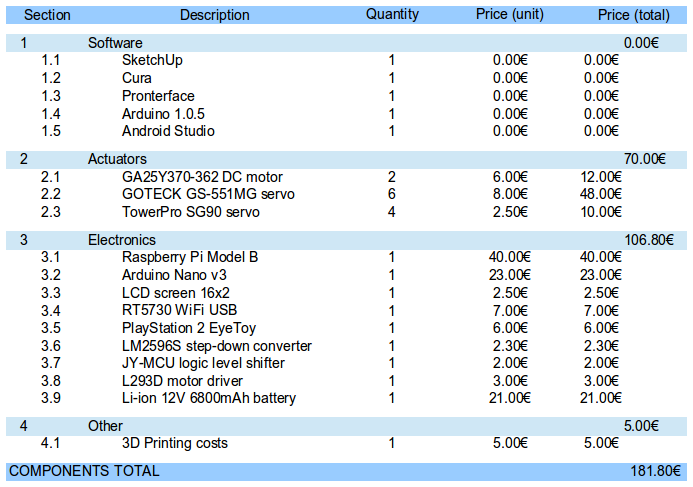
\includegraphics[width=16cm]{appendices/Presupuesto.png}
\bigskip


The robot's components cost is of 181.80 \euro. \\

However, this only takes into account the cost of replicating the robot, not the actual cost of developping the project. In order to get the total cost for this project the engineer's man hours cost must be included, and these can be seen in the previous appendix. \\

The total number of hours being XXXXXXXXX at an hourly rate of 8\euro, the cost of man hours is 

Therefore, the project's total cost is $181.80+$
\end{appendices}


\bibliographystyle{plain}
\bibliography{Conclusion/mybib}

\end{document}
